\chapter{求解误差、正则化与方法选择}
\label{chap:solution-error-regularization}

前几章给出了多条求解路线：直接分解、定常迭代、Krylov子空间法与行列投影法。每条路线最后都交出一个向量，但交出来的向量并不都同样可信。设两列几乎平行的矩阵配上略有误差的观测：精确地解出方程，系数可能离真实值很远；换成另一种算法，可能连这个精确解也没有算准；迭代法提前停下，又多出一份截断误差。即使残差已经很小，也不能直接断言系数可靠。

本章回答三个问题：算出的解能相信多少，问题本身太敏感时怎么办，以及在多种方法都可用时怎样选择。

第~\ref{sec:ls-numerical-sensitivity}节先把误差的来源分开。数据误差经问题本身放大，用有限扰动界与条件数度量；近似解的质量用残差、前向误差与后向误差判断；最小二乘的系数、拟合值与残差敏感程度不同；矩阵的秩一旦变化，伪逆可能不连续，数值秩要结合误差水平确定。这里用到第~\ref{chap:condition-and-spectral-perturbation}章的条件数与奇异值扰动界，以及第~\ref{chap:linear-solution-selection}章的伪逆与选解。

第~\ref{sec:ls-truncated-svd-ridge}节处理敏感性本身无法由算法消除的情形。岭回归与Tikhonov正则化在目标中加入惩罚，谱截断正则化舍弃小奇异值方向，二者都主动改变求解目标，用拟合误差与偏差换取稳定。截断所用矩阵的最佳低秩性质留到第~\ref{chap:matrix-approximation}章。

第~\ref{sec:ls-method-selection}节在前两节建立的误差标准下，把第~\ref{chap:direct-linear-solvers}—\ref{chap:row-projection-methods}章的方法放回同一组问题中比较：先确定求解目标，再看矩阵条件、计算开销与收敛速度、数值稳定性，最后给出典型问题的取舍。本章的误差分析都针对有限大小的扰动；扰动趋于零时的局部线性化观点在第~\ref{chap:differential-perturbation-analysis}章讨论。

\section{解的误差与敏感性}
\label{sec:ls-numerical-sensitivity}

求解目标确定、算法也给出结果以后，还要回答算出的结果能相信多少。本节分四方面讨论：数据的扰动怎样传到解，算出的近似解怎样用残差判断，最小二乘的不同输出各有多敏感，以及矩阵的秩变化时伪逆怎样变化。

讨论每种误差，都要先说清以什么为参照、允许修改哪些数据。比较两个精确解时，修改的是$\bm A$或$\bm b$，参照是原问题的精确解。用残差判断近似解时，数据不改，参照是未知的真解。后向误差则反过来问：数据至少要改多少，近似解才成为修改后问题的精确解。

以下结论都由精确方程、范数估计和奇异值性质建立，扰动可以有有限大小；所用的条件数与奇异值扰动界来自第~\ref{chap:condition-and-spectral-perturbation}章。扰动趋于零时的局部观点留到后文：第~\ref{chap:matrix-differentiation}章建立逆矩阵等运算的微分公式，第~\ref{chap:differential-perturbation-analysis}章再从同样的精确关系中提取解映射的一阶响应，讨论局部条件数与一阶近似的余项。

\subsection{系数矩阵与右端项的扰动}
\label{sec:ls-equation-sensitivity}

方程的数据常常来自测量或前一步计算，本身就带有误差。本小节回答：数据改变一点，方程的精确解改变多少。这里比较的是两个精确解，与算法和舍入无关，所以放大完全来自问题本身。

本小节设$\bm A\in\mathbb R^{d\times d}$可逆，$\bm b\ne\bm0$，精确解为$\bm x_\star=\bm A^{-1}\bm b$。向量范数与它诱导的矩阵范数始终取同一种，记
\[
 \kappa(\bm A)=\lVert\bm A\rVert\,\lVert\bm A^{-1}\rVert .
\]
用二范数时写作$\kappa_2(\bm A)$。

\paragraph{右端扰动}
先固定$\bm A$，只把右端改为$\bm b+\Delta\bm b$，记新解为$\bm x_\star+\Delta\bm x$。我们关心的是解的相对变化与右端的相对变化之比，它说明右端的误差被放大了多少倍。

新旧两个方程分别为
\[
 \bm A(\bm x_\star+\Delta\bm x)=\bm b+\Delta\bm b,\qquad \bm A\bm x_\star=\bm b .
\]
两式相减，得到
\begin{equation}
 \bm A\,\Delta\bm x=\Delta\bm b,\qquad\text{即}\qquad \Delta\bm x=\bm A^{-1}\Delta\bm b .
 \label{eq:ls-rhs-perturbation-exact}
\end{equation}
推导中没有任何近似，所以这个关系对任意大小的$\Delta\bm b$都精确成立。

对它取范数，得到解的绝对变化的界
\[
 \lVert\Delta\bm x\rVert\leq\lVert\bm A^{-1}\rVert\,\lVert\Delta\bm b\rVert .
\]
要换成相对变化，还需要用$\lVert\bm b\rVert$估计$\lVert\bm x_\star\rVert$。由$\bm b=\bm A\bm x_\star$，
\[
 \lVert\bm b\rVert\leq\lVert\bm A\rVert\,\lVert\bm x_\star\rVert,\qquad\text{即}\qquad \frac1{\lVert\bm x_\star\rVert}\leq\frac{\lVert\bm A\rVert}{\lVert\bm b\rVert}.
\]
两个不等式相乘，得到相对误差界
\begin{equation}
 \frac{\lVert\Delta\bm x\rVert}{\lVert\bm x_\star\rVert}\leq\kappa(\bm A)\,\frac{\lVert\Delta\bm b\rVert}{\lVert\bm b\rVert}.
 \label{eq:ls-rhs-relative-error-bound}
\end{equation}
这就是第~\ref{sec:ls-matrix-condition-number}节的条件数界（定理~\ref{thm:matrix-analysis-condition-number-bound}）：条件数是右端相对误差的最大放大倍数。

哪些方向上的右端误差放大得最多，可以由奇异值分解读出。设$\bm A=\sum_{i=1}^d\sigma_i\bm u_i\bm v_i^\top$，把右端的变化按左奇异向量展开，
\[
 \Delta\bm b=\sum_{i=1}^d\beta_i\bm u_i,\qquad \beta_i=\bm u_i^\top\Delta\bm b .
\]
由于$\bm A^{-1}=\sum_i\sigma_i^{-1}\bm v_i\bm u_i^\top$，解的变化为
\begin{equation}
 \Delta\bm x=\bm A^{-1}\Delta\bm b=\sum_{i=1}^d\frac{\beta_i}{\sigma_i}\,\bm v_i .
 \label{eq:ls-rhs-perturbation-svd}
\end{equation}
沿$\bm u_i$的误差分量被放大$1/\sigma_i$倍，并转到$\bm v_i$方向上。误差落在最小奇异值对应的方向上时，放大最多。下面的例子在精确算术中计算，比较一个良态矩阵和一个两列接近同向的矩阵。

\begin{example}[良态矩阵与近平行列矩阵]
\label{ex:ls-rhs-perturbation-near-parallel}
先看一个良态的对照，取以下数据：
\[
 \bm A_1=\begin{bmatrix}2&0\\0&1\end{bmatrix},\qquad \bm b=\begin{bmatrix}2\\1\end{bmatrix}.
\]
精确解为$\bm x_\star=(1,1)^\top$，$\kappa_2(\bm A_1)=2$。把右端的第二个分量改为$1.01$，即$\Delta\bm b=(0,0.01)^\top$，则解的变化为
\[
 \Delta\bm x=\bm A_1^{-1}\Delta\bm b=\begin{bmatrix}0\\0.01\end{bmatrix},
\]
新解为$(1,1.01)^\top$。右端与解的相对变化分别为
\[
 \frac{\lVert\Delta\bm b\rVert_2}{\lVert\bm b\rVert_2}=\frac{0.01}{\sqrt5}\approx0.00447,\qquad
 \frac{\lVert\Delta\bm x\rVert_2}{\lVert\bm x_\star\rVert_2}=\frac{0.01}{\sqrt2}\approx0.00707,
\]
放大约$1.58$倍，不超过$\kappa_2(\bm A_1)=2$。

再取两列接近同向的矩阵
\[
 \bm A_2=\begin{bmatrix}1&1\\0&\varepsilon\end{bmatrix},\qquad \varepsilon=10^{-2},
\]
它的逆矩阵为
\[
 \bm A_2^{-1}=\begin{bmatrix}1&-1/\varepsilon\\0&1/\varepsilon\end{bmatrix}.
\]
右端取$\bm b=(2,0)^\top$，解为$\bm x_\star=(2,0)^\top$。把右端的第二个分量改为$\eta$，解的变化按元素为
\[
 \Delta\bm x=\bm A_2^{-1}\begin{bmatrix}0\\\eta\end{bmatrix}=\begin{bmatrix}-\eta/\varepsilon\\\eta/\varepsilon\end{bmatrix}.
\]
取$\eta=0.01$，得$\Delta\bm x=(-1,1)^\top$，解由$(2,0)^\top$变为$(1,1)^\top$。右端与解的相对变化分别为
\[
 \frac{\lVert\Delta\bm b\rVert_2}{\lVert\bm b\rVert_2}=\frac{0.01}{2}=0.005,\qquad
 \frac{\lVert\Delta\bm x\rVert_2}{\lVert\bm x_\star\rVert_2}=\frac{\sqrt2}{2}\approx0.707,
\]
放大约$141$倍。

这个倍数可以与条件数比较。$\bm A_2^\top\bm A_2=\left[\begin{smallmatrix}1&1\\1&1+\varepsilon^2\end{smallmatrix}\right]$的特征值是$\sigma_{\max}^2$与$\sigma_{\min}^2$，由迹与行列式得
\[
 \sigma_{\max}^2+\sigma_{\min}^2=2+\varepsilon^2,\qquad \sigma_{\max}\sigma_{\min}=\varepsilon .
\]
解出
\[
 \sigma_{\max}\approx1.41423,\qquad \sigma_{\min}\approx0.0070710,
\]
所以$\kappa_2(\bm A_2)\approx200$。

实际倍数$141$没有达到$200$，差别来自$\bm b$：界中用$\lVert\bm A_2\rVert_2\approx1.414$估计$\lVert\bm b\rVert_2/\lVert\bm x_\star\rVert_2$，而这里该比值为$1$。

放大的方向也可以由奇异向量看出。数值计算给出
\[
 \bm v_{\min}\approx\begin{bmatrix}0.7071\\-0.7071\end{bmatrix},\qquad
 \bm u_{\min}\approx\begin{bmatrix}0.0050\\-1.0000\end{bmatrix}.
\]
$\Delta\bm b=(0,0.01)^\top$几乎全部落在$\bm u_{\min}$上，系数$\beta_{\min}\approx-0.0100$，而沿另一方向的系数只有约$5\times10^{-5}$。于是
\[
 \Delta\bm x\approx\frac{\beta_{\min}}{\sigma_{\min}}\,\bm v_{\min}\approx-1.4142\,\bm v_{\min}\approx\begin{bmatrix}-1\\1\end{bmatrix}.
\]
解的变化正沿着$\bm v_{\min}$，两个系数此增彼减。图~\ref{fig:matrix-analysis-coefficient-sensitivity}画出了$\varepsilon$减小时这种分裂怎样加剧。
\end{example}

\begin{figure}
 \centering
 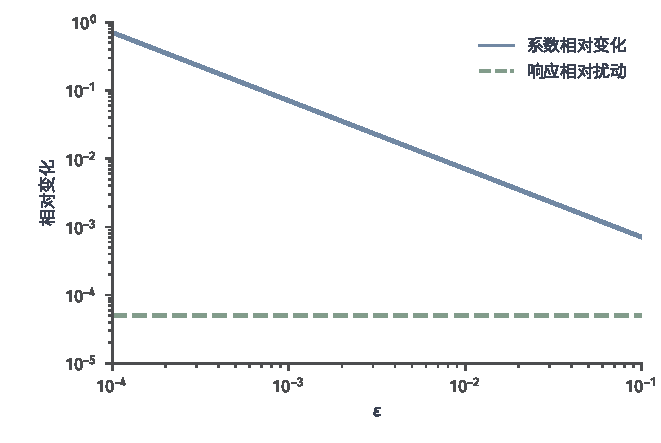
\includegraphics[width=0.92\linewidth]{figures/00-shared/mathematical-preliminaries-upper/02-linear-spaces/matplotlib/matrix-analysis-coefficient-sensitivity/figure.pdf}
 \caption{近平行列的系数分裂。取$\bm A_2=\left[\begin{smallmatrix}1&1\\0&\varepsilon\end{smallmatrix}\right]$、$\bm b=(2,0)^\top$，固定右端扰动$\Delta\bm b=(0,10^{-4})^\top$。蓝线为系数相对变化$\lVert\Delta\bm x\rVert_2/\lVert\bm x\rVert_2$，绿虚线为右端相对扰动$\lVert\Delta\bm b\rVert_2/\lVert\bm b\rVert_2$。两个系数沿相反方向偏离$(2,0)^\top$，变化量随$1/\varepsilon$增长。}
 \label{fig:matrix-analysis-coefficient-sensitivity}
\end{figure}

\paragraph{系数矩阵的扰动}
\label{sec:ls-inverse-sensitivity}%
系数矩阵的元素也可能带误差。设扰动后的矩阵为$\bm B=\bm A+\bm E$。与右端扰动不同，这时会出现一个新问题：$\bm B$甚至可能不可逆，例如$\bm E=-\bm A$。所以要先确定扰动多小时$\bm B$一定可逆，再估计$\bm B^{-1}$离$\bm A^{-1}$多远。

直观地看，$\bm E$是否算“小”，不能只看它本身的大小，还要看$\bm A$离奇异有多远。$\bm A^{-1}$的范数越大，$\bm A$越接近奇异，能容忍的扰动越小。下面的定理用乘积$\bm A^{-1}\bm E$或$\lVert\bm A^{-1}\rVert\lVert\bm E\rVert$来衡量扰动。

\begin{theorem}[逆矩阵的有限扰动]
\label{thm:ls-inverse-finite-perturbation}
设$\bm A\in\mathbb R^{d\times d}$可逆，$\bm B=\bm A+\bm E$。
\begin{enumerate}
 \item 若$\lVert\bm A^{-1}\bm E\rVert<1$，则$\bm B$可逆，
 \begin{equation}
  \lVert\bm B^{-1}\rVert\leq\frac{\lVert\bm A^{-1}\rVert}{1-\lVert\bm A^{-1}\bm E\rVert},
  \label{eq:ls-inverse-norm-bound}
 \end{equation}
 且
 \begin{equation}
  \bm B^{-1}-\bm A^{-1}=-\bm B^{-1}\bm E\,\bm A^{-1}.
  \label{eq:ch06-inverse-finite-perturbation}
 \end{equation}
 \item 若$q=\lVert\bm A^{-1}\rVert\lVert\bm E\rVert<1$，则第1条适用，并且
 \begin{equation}
  \frac{\lVert\bm B^{-1}-\bm A^{-1}\rVert}{\lVert\bm A^{-1}\rVert}
  \leq\frac{q}{1-q},\qquad q=\kappa(\bm A)\frac{\lVert\bm E\rVert}{\lVert\bm A\rVert}.
  \label{eq:ls-inverse-relative-perturbation-bound}
 \end{equation}
\end{enumerate}
\end{theorem}
\begin{proof}
先证第1条中的可逆性。设$\bm B\bm x=\bm0$，即$\bm A\bm x=-\bm E\bm x$，两边左乘$\bm A^{-1}$并取范数，
\[
 \bm x=-\bm A^{-1}\bm E\bm x,\qquad \lVert\bm x\rVert\leq\lVert\bm A^{-1}\bm E\rVert\,\lVert\bm x\rVert .
\]
由于$\lVert\bm A^{-1}\bm E\rVert<1$，只能$\lVert\bm x\rVert=0$。方阵$\bm B$的零空间只含零向量，故$\bm B$可逆。

再估计$\lVert\bm B^{-1}\rVert$。对任意$\bm y$，令$\bm x=\bm B^{-1}\bm y$，则$\bm A\bm x+\bm E\bm x=\bm y$。左乘$\bm A^{-1}$并取范数，
\[
 \begin{gathered}
 \bm x=\bm A^{-1}\bm y-\bm A^{-1}\bm E\bm x,\\
 \lVert\bm x\rVert\leq\lVert\bm A^{-1}\rVert\,\lVert\bm y\rVert+\lVert\bm A^{-1}\bm E\rVert\,\lVert\bm x\rVert .
 \end{gathered}
\]
把含$\lVert\bm x\rVert$的项移到左边，
\[
 \bigl(1-\lVert\bm A^{-1}\bm E\rVert\bigr)\lVert\bm B^{-1}\bm y\rVert\leq\lVert\bm A^{-1}\rVert\,\lVert\bm y\rVert .
\]
对所有$\lVert\bm y\rVert=1$取上确界，即得$\lVert\bm B^{-1}\rVert$的界。恒等式由$\bm A-\bm B=-\bm E$得到：
\[
 \begin{aligned}
 \bm B^{-1}-\bm A^{-1}&=\bm B^{-1}\bm A\bm A^{-1}-\bm B^{-1}\bm B\bm A^{-1}\\
 &=\bm B^{-1}(\bm A-\bm B)\bm A^{-1}=-\bm B^{-1}\bm E\bm A^{-1}.
 \end{aligned}
\]

第2条中，$\lVert\bm A^{-1}\bm E\rVert\leq\lVert\bm A^{-1}\rVert\lVert\bm E\rVert=q<1$，所以第1条适用，并有$\lVert\bm B^{-1}\rVert\leq\lVert\bm A^{-1}\rVert/(1-q)$。对式~\eqref{eq:ch06-inverse-finite-perturbation}取范数，
\[
 \begin{aligned}
 \lVert\bm B^{-1}-\bm A^{-1}\rVert&\leq\lVert\bm B^{-1}\rVert\,\lVert\bm E\rVert\,\lVert\bm A^{-1}\rVert\\
 &\leq\frac{\lVert\bm A^{-1}\rVert^2\lVert\bm E\rVert}{1-q}=\frac{q}{1-q}\,\lVert\bm A^{-1}\rVert .
 \end{aligned}
\]
两边除以$\lVert\bm A^{-1}\rVert$即得。最后，
\[
 q=\lVert\bm A\rVert\lVert\bm A^{-1}\rVert\cdot\frac{\lVert\bm E\rVert}{\lVert\bm A\rVert}=\kappa(\bm A)\frac{\lVert\bm E\rVert}{\lVert\bm A\rVert}.
\]
\end{proof}

界的分子$q$是条件数乘矩阵的相对扰动，分母$1-q$是到可逆性保证边界的余量。$q$越接近$1$，余量越小，界就越大。

\begin{example}[一次系数扰动]
\label{ex:ls-inverse-perturbation-numeric}
取示例~\ref{ex:ls-stationary-running-example}的矩阵，并只扰动它的右下角元素：
\[
 \bm A=\begin{bmatrix}4&1\\1&3\end{bmatrix},\qquad
 \bm E=\begin{bmatrix}0&0\\0&1/2\end{bmatrix}.
\]
扰动后的矩阵为
\[
 \bm B=\bm A+\bm E=\begin{bmatrix}4&1\\1&7/2\end{bmatrix}.
\]
两个逆矩阵分别为
\[
 \bm A^{-1}=\frac1{11}\begin{bmatrix}3&-1\\-1&4\end{bmatrix},\qquad
 \bm B^{-1}=\frac1{26}\begin{bmatrix}7&-2\\-2&8\end{bmatrix}.
\]
直接相减，得
\[
 \bm B^{-1}-\bm A^{-1}=\frac1{286}\begin{bmatrix}-1&4\\4&-16\end{bmatrix}.
\]
按恒等式~\eqref{eq:ch06-inverse-finite-perturbation}计算$-\bm B^{-1}\bm E\bm A^{-1}$，得到同一个矩阵。它是一个秩一矩阵，
\[
 \bm B^{-1}-\bm A^{-1}=-\frac1{286}\begin{bmatrix}1\\-4\end{bmatrix}\begin{bmatrix}1&-4\end{bmatrix},
\]
谱范数为$17/286\approx0.0594$。

在谱范数下，$\bm A$的特征值为$(7\pm\sqrt5)/2$，所以
\[
 \lVert\bm A\rVert_2\approx4.618,\qquad \lVert\bm A^{-1}\rVert_2\approx0.4198,\qquad \kappa_2(\bm A)\approx1.939 .
\]
于是
\[
 q=\lVert\bm A^{-1}\rVert_2\lVert\bm E\rVert_2\approx0.4198\times0.5\approx0.210 .
\]
定理给出的界与实际的相对变化分别为
\[
 \frac{q}{1-q}\approx0.266,\qquad
 \frac{\lVert\bm B^{-1}-\bm A^{-1}\rVert_2}{\lVert\bm A^{-1}\rVert_2}\approx\frac{0.0594}{0.4198}\approx0.142 .
\]
第1条的范数界也成立。这里
\[
 \lVert\bm A^{-1}\bm E\rVert_2=\frac{\sqrt{17}}{22}\approx0.187,
\]
界为$0.4198/(1-0.187)\approx0.517$，而$\lVert\bm B^{-1}\rVert_2\approx0.368$。
\end{example}

这个界可以取到。取对角矩阵
\[
 \bm A=\begin{bmatrix}1&0\\0&\varepsilon\end{bmatrix},\qquad
 \bm E=\begin{bmatrix}0&0\\0&-\delta\end{bmatrix},\qquad 0<\delta<\varepsilon<1 .
\]
在谱范数下$\lVert\bm A^{-1}\rVert_2=1/\varepsilon$，$q=\delta/\varepsilon$。逆矩阵只在右下角改变，
\[
 \bm B^{-1}-\bm A^{-1}=\begin{bmatrix}0&0\\0&\dfrac1{\varepsilon-\delta}-\dfrac1\varepsilon\end{bmatrix}.
\]
右下角元素等于$\delta/(\varepsilon(\varepsilon-\delta))$，所以相对变化为
\[
 \frac{\lVert\bm B^{-1}-\bm A^{-1}\rVert_2}{\lVert\bm A^{-1}\rVert_2}=\frac{\delta}{\varepsilon-\delta}=\frac q{1-q}.
\]
例如$\varepsilon=0.1$、$\delta=0.05$时，$q=0.5$，逆矩阵的相对变化恰为$1$；$\delta\to\varepsilon$时它无界，因为$\bm B$趋于奇异。

反过来，$q\geq1$只表示定理不再给出保证，并不意味着$\bm B$已经奇异。例如$\bm E=\bm A$时$q=\kappa(\bm A)\geq1$，而$\bm B=2\bm A$仍可逆。

\paragraph{矩阵与右端同时扰动}
实际问题中矩阵与右端往往同时带误差。这时扰动后的方程为
\[
 (\bm A+\bm E)(\bm x_\star+\Delta\bm x)=\bm b+\Delta\bm b .
\]
展开左边，得
\[
 \bm A\bm x_\star+\bm A\Delta\bm x+\bm E\bm x_\star+\bm E\Delta\bm x=\bm b+\Delta\bm b .
\]
减去原方程$\bm A\bm x_\star=\bm b$，整理得到精确关系
\begin{equation}
 (\bm A+\bm E)\Delta\bm x=\Delta\bm b-\bm E\bm x_\star .
 \label{eq:ls-joint-perturbation-exact}
\end{equation}

式~\eqref{eq:ls-joint-perturbation-exact}说明，解的变化由两部分驱动：一是右端的变化$\Delta\bm b$，二是矩阵的变化作用在原解上产生的$\bm E\bm x_\star$。在定理~\ref{thm:ls-inverse-finite-perturbation}的条件下$\bm A+\bm E$可逆，于是
\[
 \Delta\bm x=(\bm A+\bm E)^{-1}(\Delta\bm b-\bm E\bm x_\star).
\]
下面的定理把两类扰动的相对大小合起来，估计解的相对变化。

\begin{theorem}[矩阵与右端同时扰动时的解误差]
\label{thm:ls-linear-system-perturbation}
设$\rho_A=\lVert\bm E\rVert/\lVert\bm A\rVert$，$\rho_b=\lVert\Delta\bm b\rVert/\lVert\bm b\rVert$。若$\kappa(\bm A)\rho_A<1$，则$\bm A+\bm E$可逆，且
\begin{equation}
 \frac{\lVert\Delta\bm x\rVert}{\lVert\bm x_\star\rVert}
 \leq\frac{\kappa(\bm A)\,(\rho_A+\rho_b)}{1-\kappa(\bm A)\rho_A}.
 \label{eq:matrix-analysis-linear-system-perturbation}
\end{equation}
\end{theorem}
\begin{proof}
由于$\kappa(\bm A)\rho_A=\lVert\bm A^{-1}\rVert\lVert\bm E\rVert$，可逆性由定理~\ref{thm:ls-inverse-finite-perturbation}第2条得到。把式~\eqref{eq:ls-joint-perturbation-exact}中的$\bm E\Delta\bm x$移到右边，再左乘$\bm A^{-1}$，
\[
 \Delta\bm x=\bm A^{-1}\bigl(\Delta\bm b-\bm E\bm x_\star-\bm E\Delta\bm x\bigr).
\]
取范数，得
\[
 \lVert\Delta\bm x\rVert\leq\lVert\bm A^{-1}\rVert\bigl(\lVert\Delta\bm b\rVert+\lVert\bm E\rVert\lVert\bm x_\star\rVert+\lVert\bm E\rVert\lVert\Delta\bm x\rVert\bigr).
\]
把含$\lVert\Delta\bm x\rVert$的项移到左边，
\[
 \begin{aligned}
 &\bigl(1-\lVert\bm A^{-1}\rVert\lVert\bm E\rVert\bigr)\lVert\Delta\bm x\rVert\\
 &\qquad\leq\lVert\bm A^{-1}\rVert\,\lVert\Delta\bm b\rVert+\lVert\bm A^{-1}\rVert\,\lVert\bm E\rVert\,\lVert\bm x_\star\rVert .
 \end{aligned}
\]
右边两项分别估计。由$\lVert\bm b\rVert\leq\lVert\bm A\rVert\lVert\bm x_\star\rVert$，
\[
 \begin{gathered}
 \lVert\bm A^{-1}\rVert\,\lVert\Delta\bm b\rVert=\lVert\bm A^{-1}\rVert\,\rho_b\lVert\bm b\rVert\leq\kappa(\bm A)\rho_b\lVert\bm x_\star\rVert,\\
 \lVert\bm A^{-1}\rVert\,\lVert\bm E\rVert\,\lVert\bm x_\star\rVert=\kappa(\bm A)\rho_A\lVert\bm x_\star\rVert .
 \end{gathered}
\]
左边的系数为$1-\kappa(\bm A)\rho_A>0$。两边除以它与$\lVert\bm x_\star\rVert$，即得式~\eqref{eq:matrix-analysis-linear-system-perturbation}。
\end{proof}

这个界的结构是：两类相对扰动先相加，再被条件数放大，最后除以到奇异边界的余量。$\bm E=\bm0$时$\rho_A=0$，它退回只扰动右端的界。

\begin{example}[矩阵与右端同时扰动]
\label{ex:ls-joint-perturbation-numeric}
沿用示例~\ref{ex:ls-inverse-perturbation-numeric}的$\bm A$与$\bm E$，取$\bm b=(1,2)^\top$，精确解为$\bm x_\star=(1/11,7/11)^\top$。矩阵变化作用在原解上，得
\[
 \bm E\bm x_\star=\begin{bmatrix}0\\7/22\end{bmatrix}.
\]
先取右端变化$\Delta\bm b=(0,-1/4)^\top$。式~\eqref{eq:ls-joint-perturbation-exact}的右端为
\[
 \Delta\bm b-\bm E\bm x_\star=\begin{bmatrix}0\\-25/44\end{bmatrix}.
\]
左乘$\bm B^{-1}$，得解的变化
\[
 \Delta\bm x=\bm B^{-1}\begin{bmatrix}0\\-25/44\end{bmatrix}=\begin{bmatrix}25/572\\-25/143\end{bmatrix}.
\]
在二范数下，$\lVert\bm x_\star\rVert_2\approx0.6428$，$\lVert\Delta\bm x\rVert_2\approx0.1802$，相对变化约为$0.280$。

再看定理给出的界。两类相对扰动为
\[
 \rho_A=\frac{0.5}{4.618}\approx0.108,\qquad \rho_b=\frac{0.25}{\sqrt5}\approx0.112,
\]
$\kappa_2(\bm A)\rho_A\approx0.210<1$，所以界为
\[
 \frac{1.939\times(0.108+0.112)}{1-0.210}\approx0.540 .
\]
实际变化$0.280$不超过它。

若右端变化改为$\Delta\bm b=(0,1/4)^\top$，两类扰动的大小不变，界仍是$0.540$。但这时
\[
 \Delta\bm b-\bm E\bm x_\star=\begin{bmatrix}0\\-3/44\end{bmatrix},
\]
两项部分抵消，解的变化只有
\[
 \Delta\bm x=\begin{bmatrix}3/572\\-3/143\end{bmatrix},
\]
相对变化约为$0.034$。

定理只用到扰动的大小，看不到这种方向上的抵消，所以它给出的是最坏情形的估计。
\end{example}

第~\ref{sec:multivariable-inverse-perturbation}节还会从同一精确式~\eqref{eq:ls-joint-perturbation-exact}提取解映射的一阶响应；这里得到的结论不依赖扰动趋于零，对完整的有限变化有效。

\subsection{残差、前向误差与后向误差}
\label{sec:ls-numerical-stability}

\paragraph{残差与前向误差}
上一小节比较的是两个精确解。实际计算只给出一个近似解$\tilde{\bm x}$，真解$\bm x_\star$未知，无法直接算出误差$\tilde{\bm x}-\bm x_\star$。能直接算出的是残差
\[
 \bm r=\bm b-\bm A\tilde{\bm x},
\]
它衡量$\tilde{\bm x}$在多大程度上满足方程。要问的是：残差小，能否说明误差也小。

把$\bm b=\bm A\bm x_\star$代入残差，得
\begin{equation}
 \bm r=\bm A\bm x_\star-\bm A\tilde{\bm x}=\bm A(\bm x_\star-\tilde{\bm x}),\qquad\text{即}\qquad \bm x_\star-\tilde{\bm x}=\bm A^{-1}\bm r .
 \label{eq:ls-error-residual-identity}
\end{equation}
这与右端扰动的关系$\Delta\bm x=\bm A^{-1}\Delta\bm b$形式相同：$\tilde{\bm x}$恰是右端改为$\bm b-\bm r$的方程的精确解，残差扮演了右端误差的角色。于是由右端扰动的条件数界，
\begin{equation}
 \frac{\lVert\tilde{\bm x}-\bm x_\star\rVert}{\lVert\bm x_\star\rVert}\leq\kappa(\bm A)\frac{\lVert\bm r\rVert}{\lVert\bm b\rVert}.
 \label{eq:ls-residual-error-bound}
\end{equation}

条件数大时，这个界允许小残差对应大误差，而且这种情形确实会发生。取以下方程：
\[
 \bm A=\begin{bmatrix}1&0\\0&\varepsilon\end{bmatrix},\qquad
 \bm b=\begin{bmatrix}1\\\varepsilon\end{bmatrix}.
\]
它的精确解与一个近似解分别为
\[
 \bm x_\star=\begin{bmatrix}1\\1\end{bmatrix},\qquad
 \tilde{\bm x}=\begin{bmatrix}1\\0\end{bmatrix}.
\]
近似解的残差为$\bm r=(0,\varepsilon)^\top$，随$\varepsilon\to0$趋于零；相对误差却始终是
\[
 \frac{\lVert\tilde{\bm x}-\bm x_\star\rVert_2}{\lVert\bm x_\star\rVert_2}=\frac1{\sqrt2}.
\]
这并不与上面的界矛盾：$\kappa_2(\bm A)=1/\varepsilon$，界的右端为$1/\sqrt{1+\varepsilon^2}$，仍不小于$1/\sqrt2$。病态时，小残差什么也不保证。

因此要区分两种误差。近似解离真解多远，即$\lVert\tilde{\bm x}-\bm x_\star\rVert$或其相对量，称为\term{前向误差}（forward error）。至少要把数据修改多少，才能让$\tilde{\bm x}$成为修改后问题的精确解，称为\term{后向误差}（backward error）。前者需要真解才能算；后者只用数据和近似解就能算，下面先说明它的度量方式。

\paragraph{后向误差的度量}
后向误差的想法是：数据本身只准确到某个误差水平，如果$\tilde{\bm x}$恰好是一个与原数据相差不超过这一水平的问题的精确解，就不能再要求更多。它的大小取决于允许怎样修改数据。

范数型模型只限制修改量的范数：允许的修改满足
\begin{equation}
 \lVert\Delta\bm A\rVert\leq\epsilon\lVert\bm A\rVert,\qquad \lVert\Delta\bm b\rVert\leq\epsilon\lVert\bm b\rVert,
 \label{eq:ls-normwise-backward-model}
\end{equation}
并且使$\tilde{\bm x}$成为精确解，
\begin{equation}
 (\bm A+\Delta\bm A)\tilde{\bm x}=\bm b+\Delta\bm b .
 \label{eq:ls-backward-exact-condition}
\end{equation}
满足这两个要求的最小$\epsilon$记作$\eta(\tilde{\bm x})$。在二范数下，它可以由残差直接算出。

\begin{theorem}[范数型后向误差]
\label{thm:ls-backward-error-formulas}
设$\bm A\in\mathbb R^{m\times d}$，$\tilde{\bm x}\in\mathbb R^d$，$\bm r=\bm b-\bm A\tilde{\bm x}$，且$s=\lVert\bm A\rVert_2\lVert\tilde{\bm x}\rVert_2+\lVert\bm b\rVert_2>0$。则在二范数下
\begin{equation}
 \eta_2(\tilde{\bm x})=\frac{\lVert\bm r\rVert_2}{\lVert\bm A\rVert_2\lVert\tilde{\bm x}\rVert_2+\lVert\bm b\rVert_2},
 \label{eq:ls-normwise-backward-error}
\end{equation}
并且下确界可以取到。
\end{theorem}
\begin{proof}
先证下界。若$(\bm A+\Delta\bm A)\tilde{\bm x}=\bm b+\Delta\bm b$，且两项修改的相对大小都不超过$\epsilon$，把$\bm A\tilde{\bm x}$与$\Delta\bm b$分别移到两边，得
\[
 \bm r=\bm b-\bm A\tilde{\bm x}=\Delta\bm A\tilde{\bm x}-\Delta\bm b .
\]
取范数，
\[
 \lVert\bm r\rVert_2\leq\lVert\Delta\bm A\rVert_2\lVert\tilde{\bm x}\rVert_2+\lVert\Delta\bm b\rVert_2
 \leq\epsilon\bigl(\lVert\bm A\rVert_2\lVert\tilde{\bm x}\rVert_2+\lVert\bm b\rVert_2\bigr)=\epsilon s,
\]
所以$\epsilon\geq\lVert\bm r\rVert_2/s$。

再构造一组达到下界的修改。$\tilde{\bm x}=\bm0$时$s=\lVert\bm b\rVert_2$，$\bm r=\bm b$，取$\Delta\bm A=\bm0$、$\Delta\bm b=-\bm b$即可，其相对大小为$1=\lVert\bm r\rVert_2/s$。$\tilde{\bm x}\ne\bm0$时取
\[
 \Delta\bm A=\frac{\lVert\bm A\rVert_2}{s\lVert\tilde{\bm x}\rVert_2}\,\bm r\tilde{\bm x}^\top,\qquad
 \Delta\bm b=-\frac{\lVert\bm b\rVert_2}{s}\,\bm r .
\]
由$\tilde{\bm x}^\top\tilde{\bm x}=\lVert\tilde{\bm x}\rVert_2^2$，
\[
 \Delta\bm A\tilde{\bm x}-\Delta\bm b=\frac{\lVert\bm A\rVert_2\lVert\tilde{\bm x}\rVert_2}{s}\,\bm r+\frac{\lVert\bm b\rVert_2}{s}\,\bm r=\bm r,
\]
即$(\bm A+\Delta\bm A)\tilde{\bm x}=\bm b+\Delta\bm b$。秩一矩阵$\bm r\tilde{\bm x}^\top$的谱范数为$\lVert\bm r\rVert_2\lVert\tilde{\bm x}\rVert_2$，所以
\[
 \frac{\lVert\Delta\bm A\rVert_2}{\lVert\bm A\rVert_2}=\frac{\lVert\bm r\rVert_2}{s},\qquad
 \frac{\lVert\Delta\bm b\rVert_2}{\lVert\bm b\rVert_2}=\frac{\lVert\bm r\rVert_2}{s},
\]
两项的相对大小都等于下界。
\end{proof}

分母为零只发生在$\bm b=\bm0$且$\tilde{\bm x}=\bm0$时，这时$\tilde{\bm x}$已是精确解。

这个公式也解释了迭代法的停止准则。若只允许修改右端，即要求$\Delta\bm A=\bm0$，则$\Delta\bm b=-\bm r$是唯一的选择，后向误差就是相对残差$\lVert\bm r\rVert_2/\lVert\bm b\rVert_2$。允许同时修改$\bm A$时分母更大，所以
\begin{equation}
 \eta_2(\tilde{\bm x})\leq\frac{\lVert\bm r\rVert_2}{\lVert\bm b\rVert_2}.
 \label{eq:ls-backward-error-relative-residual}
\end{equation}
第~\ref{sec:ls-stationary-stopping}节的准则$\lVert\bm r_k\rVert_2\leq\mathrm{rtol}\,\lVert\bm b\rVert_2$（取$\mathrm{atol}=0$）因此保证后向误差不超过$\mathrm{rtol}$。

范数型模型允许把$\bm A$中的零元改成非零。若希望修改保持每个元素的相对大小，可以用逐元素模型，限制
\begin{equation}
 |\Delta\bm A|\leq\epsilon|\bm A|,\qquad |\Delta\bm b|\leq\epsilon|\bm b|,
 \label{eq:ls-componentwise-backward-model}
\end{equation}
其中绝对值与不等号都逐元素取。它不允许把零元改成非零，所得的后向误差为\scite{math-golub2013matrix}
\begin{equation}
 \omega(\tilde{\bm x})=\max_i\frac{|r_i|}{\bigl(|\bm A||\tilde{\bm x}|+|\bm b|\bigr)_i},
 \label{eq:ls-componentwise-backward-error}
\end{equation}
分子分母同为零的分量记为$0$。

两种模型可以给出相差悬殊的结果。回到上面的对角例子，$\bm r=(0,\varepsilon)^\top$。范数型后向误差为
\[
 \eta_2(\tilde{\bm x})=\frac{\varepsilon}{1\cdot1+\sqrt{1+\varepsilon^2}}\approx\frac\varepsilon2 .
\]
逐元素模型的分母向量为$|\bm A||\tilde{\bm x}|+|\bm b|=(2,\varepsilon)^\top$，所以
\[
 \omega(\tilde{\bm x})=\max\Bigl(\frac02,\ \frac\varepsilon\varepsilon\Bigr)=1 .
\]
范数型模型认为只需很小的修改，因为它可以把很小的$a_{2,2}$整体改掉；逐元素模型按第二个方程自身的尺度衡量，这个方程完全没有被满足。两种模型回答不同的问题，由一种模型得到的结论不能不加说明地用于另一种。

\begin{example}[计算一次后向误差]
\label{ex:ls-backward-error-computation}
取示例~\ref{ex:ls-stationary-running-example}的方程：
\[
 \bm A=\begin{bmatrix}4&1\\1&3\end{bmatrix},\qquad
 \bm b=\begin{bmatrix}1\\2\end{bmatrix}.
\]
它的精确解为
\[
 \bm x_\star=\begin{bmatrix}1/11\\7/11\end{bmatrix}\approx\begin{bmatrix}0.0909\\0.6364\end{bmatrix}.
\]
设某个算法给出近似解$\tilde{\bm x}=(0.09,0.64)^\top$，下面计算它的范数型后向误差。

残差按元素为
\[
 \bm r=\begin{bmatrix}1-4\times0.09-0.64\\2-0.09-3\times0.64\end{bmatrix}=\begin{bmatrix}0\\-0.01\end{bmatrix}.
\]
分母要用到三个范数。由示例~\ref{ex:ls-inverse-perturbation-numeric}，$\lVert\bm A\rVert_2\approx4.618$；又
\[
 \lVert\tilde{\bm x}\rVert_2=\sqrt{0.09^2+0.64^2}\approx0.6463,\qquad \lVert\bm b\rVert_2=\sqrt5\approx2.236 .
\]
于是
\[
 s\approx4.618\times0.6463+2.236\approx5.221,\qquad
 \eta_2(\tilde{\bm x})\approx\frac{0.01}{5.221}\approx1.92\times10^{-3}.
\]

按定理中的构造，系数为$\lVert\bm A\rVert_2/(s\lVert\tilde{\bm x}\rVert_2)\approx1.369$，而$\bm r\tilde{\bm x}^\top$只有第二行非零，
\[
 \Delta\bm A\approx1.369\begin{bmatrix}0&0\\-0.0009&-0.0064\end{bmatrix}\approx\begin{bmatrix}0&0\\-0.0012&-0.0088\end{bmatrix},
\]
右端的修正为
\[
 \Delta\bm b\approx\begin{bmatrix}0\\0.0043\end{bmatrix}.
\]
验证第二个方程：
\[
 (1-0.0012)\times0.09+(3-0.0088)\times0.64\approx2.0043,
\]
正等于$2+0.0043$；第一个方程未被修改，本来就满足。所以$\tilde{\bm x}$是一个只差千分之二左右的邻近问题的精确解。
\end{example}

\paragraph{后向稳定与常用分解}
后向误差的概念适合用来评价算法。计算机中每次基本运算都带舍入，满足
\begin{equation}
 \operatorname{fl}(x\circ y)=(x\circ y)(1+\delta),\qquad |\delta|\leq u,
 \label{eq:ls-rounding-model}
\end{equation}
其中$\circ$表示加、减、乘、除之一，$u$称为\term{单位舍入}（unit roundoff），双精度时$u=2^{-53}\approx1.1\times10^{-16}$。若算法对所有合法输入算出的结果都是某个邻近问题的精确解，且后向误差不超过$u$乘一个只依赖维数的温和常数，就称算法\term{后向稳定}（backward stable）。

后向稳定只说明算法没有额外引入比数据舍入大得多的误差，并不说明答案准确。由后向误差到前向误差，还要经过问题本身的条件数，这由下面的定理给出。

\begin{theorem}[由后向误差估计前向误差]
\label{thm:ls-forward-backward-error}
设$\bm A\in\mathbb R^{d\times d}$可逆，$\bm b\ne\bm0$。若$(\bm A+\Delta\bm A)\tilde{\bm x}=\bm b+\Delta\bm b$，$\lVert\Delta\bm A\rVert\leq\eta\lVert\bm A\rVert$，$\lVert\Delta\bm b\rVert\leq\eta\lVert\bm b\rVert$，且$\kappa(\bm A)\eta<1$，则
\begin{equation}
 \frac{\lVert\tilde{\bm x}-\bm x_\star\rVert}{\lVert\bm x_\star\rVert}\leq\frac{2\kappa(\bm A)\,\eta}{1-\kappa(\bm A)\,\eta}.
 \label{eq:ls-forward-backward-error-bound}
\end{equation}
\end{theorem}
\begin{proof}
把$\tilde{\bm x}$看作扰动问题的精确解，在定理~\ref{thm:ls-linear-system-perturbation}中取$\bm E=\Delta\bm A$、$\Delta\bm x=\tilde{\bm x}-\bm x_\star$，这时$\rho_A\leq\eta$，$\rho_b\leq\eta$。式~\eqref{eq:matrix-analysis-linear-system-perturbation}的右端随$\rho_A$与$\rho_b$增大而增大（分子增大、分母减小），所以
\[
 \frac{\lVert\tilde{\bm x}-\bm x_\star\rVert}{\lVert\bm x_\star\rVert}
 \leq\frac{\kappa(\bm A)(\rho_A+\rho_b)}{1-\kappa(\bm A)\rho_A}
 \leq\frac{\kappa(\bm A)(\eta+\eta)}{1-\kappa(\bm A)\eta}.
\]
\end{proof}

回到示例~\ref{ex:ls-backward-error-computation}。那里
\[
 \kappa_2(\bm A)\eta_2\approx1.939\times0.00192\approx0.0037,
\]
定理给出
\[
 \frac{2\kappa_2\eta_2}{1-\kappa_2\eta_2}\approx0.0075 .
\]
实际误差为$\tilde{\bm x}-\bm x_\star\approx(-0.0009,0.0036)^\top$，相对前向误差为
\[
 \frac{\lVert\tilde{\bm x}-\bm x_\star\rVert_2}{\lVert\bm x_\star\rVert_2}\approx\frac{0.00375}{0.6428}\approx0.0058,
\]
不超过$0.0075$。条件数不到$2$，所以小的后向误差在这里确实带来小的前向误差。

定理说明，前向误差大约不超过条件数乘后向误差：后向误差评价算法或近似解，条件数评价问题。即使算法后向稳定，前向误差也可能达到$\kappa(\bm A)u$的量级；$\kappa(\bm A)u$接近$1$时，答案可能没有一位有效数字。第~\ref{chap:direct-linear-solvers}章各直接法的稳定性就以此为标准\scite{math-golub2013matrix}，下面逐个说明。

带部分主元的LU（第~\ref{sec:ls-lu}节）的后向误差约为$d$的低次幂乘增长因子$\rho$再乘$u$，$\rho$是消元中出现的最大元素与$\bm A$最大元素之比。部分主元使乘子的绝对值不超过$1$，但每轮元素仍可能翻倍，$\rho$最坏可达$2^{d-1}$。$d=3$时下面的矩阵就达到这个上界。每一列中待选的主元绝对值都相同，不发生行交换。第一轮把第一行加到下面两行：
\[
 \begin{bmatrix}1&0&1\\-1&1&1\\-1&-1&1\end{bmatrix}
 \;\longrightarrow\;
 \begin{bmatrix}1&0&1\\0&1&2\\0&-1&2\end{bmatrix}.
\]
第二轮把第二行加到第三行：
\[
 \begin{bmatrix}1&0&1\\0&1&2\\0&-1&2\end{bmatrix}
 \;\longrightarrow\;
 \begin{bmatrix}1&0&1\\0&1&2\\0&0&4\end{bmatrix}.
\]
最后一列依次变为$1,2,4$，$\rho=4=2^{3-1}$。

所以部分主元LU只在增长因子不大时后向稳定；这种最坏情形在实际中极少出现，计算时可以在消元中记录$\rho$加以核验。

Cholesky分解（第~\ref{sec:ls-cholesky}节）没有增长问题。由$\bm A=\bm L\bm L^\top$的对角元，
\begin{equation}
 a_{j,j}=\sum_{k\leq j}l_{j,k}^2,\qquad\text{所以}\qquad |l_{j,k}|\leq\sqrt{a_{j,j}} .
 \label{eq:ls-cholesky-element-bound}
\end{equation}
因子的元素不会超过原矩阵对角元的平方根。例如上面的$\bm A=\left[\begin{smallmatrix}4&1\\1&3\end{smallmatrix}\right]$有$l_{2,1}=1/2$、$l_{2,2}=\sqrt{11}/2\approx1.658$，都不超过$\sqrt3\approx1.732$。因此Cholesky分解对正定矩阵后向稳定。

Householder反射与Givens旋转（第~\ref{sec:ls-qr-method}节）是正交变换，保持向量长度，前面步骤引入的误差不会被后续变换放大，用它们求最小二乘解是后向稳定的。修正Gram--Schmidt不用正交矩阵作用于数据，算出的$\bm Q$在有限精度下可能偏离正交，使用时应核验$\bm Q^\top\bm Q-\bm I$或残差。

\subsection{最小二乘的敏感性与数值误差}
\label{sec:ls-ls-regularization-sensitivity}

\paragraph{三类输出的敏感性}
最小二乘问题不只输出系数。按用途不同，关心的量有三类：系数、拟合值与残差，
\begin{equation}
 \hat{\bm x}=\bm A^\dagger\bm b,\qquad \bm A\hat{\bm x}=\bm P\bm b,\qquad \hat{\bm r}=(\bm I-\bm P)\bm b,
 \label{eq:ls-ls-three-outputs}
\end{equation}
其中$\bm P=\bm A\bm A^\dagger$是到$\operatorname{range}\bm A$的正交投影（第~\ref{sec:ls-pseudoinverse}节）。本段问：右端改变时，这三类输出各改变多少。直观上，拟合值与残差都是$\bm b$的正交投影，投影不会放大向量；系数则要经过$\bm A^\dagger$，其中含有奇异值的倒数，可能被放大很多。

固定$\bm A$，把右端改为$\bm b+\Delta\bm b$。三类输出都是$\bm b$的线性函数，所以变化精确地为
\begin{equation}
 \Delta\hat{\bm x}=\bm A^\dagger\Delta\bm b,\qquad
 \Delta(\bm A\hat{\bm x})=\bm P\Delta\bm b,\qquad
 \Delta\hat{\bm r}=(\bm I-\bm P)\Delta\bm b .
 \label{eq:ls-ls-output-perturbations}
\end{equation}

后两项是$\Delta\bm b$在一对互补正交子空间上的分量，所以
\[
 \lVert\bm P\Delta\bm b\rVert_2^2+\lVert(\bm I-\bm P)\Delta\bm b\rVert_2^2=\lVert\Delta\bm b\rVert_2^2 .
\]
拟合值与残差的绝对变化都不超过$\lVert\Delta\bm b\rVert_2$。

系数则不同。设$\bm A$的秩为$r$，奇异值分解为$\bm A=\sum_{i=1}^r\sigma_i\bm u_i\bm v_i^\top$，则
\begin{equation}
 \bm A^\dagger=\sum_{i=1}^r\frac1{\sigma_i}\bm v_i\bm u_i^\top,\qquad
 \lVert\Delta\hat{\bm x}\rVert_2\leq\frac{\lVert\Delta\bm b\rVert_2}{\sigma_r},
 \label{eq:ls-ls-coefficient-sensitivity-bound}
\end{equation}
$\sigma_r$为最小正奇异值；$\Delta\bm b$沿$\bm u_r$时取等号。所以拟合得好与系数可靠是两回事。

\begin{example}[三类输出的不同变化]
\label{ex:ls-three-outputs-sensitivity}
在示例~\ref{ex:ls-rhs-perturbation-near-parallel}的$\bm A_2$下面添一个零行，得到$3\times2$的满列秩矩阵。取
\[
 \bm A=\begin{bmatrix}1&1\\0&\varepsilon\\0&0\end{bmatrix},\qquad
 \bm b=\begin{bmatrix}2\\0\\1\end{bmatrix},\qquad \varepsilon=10^{-2}.
\]
由于$\bm A^\top\bm A=\bm A_2^\top\bm A_2$，伪逆$\bm A^\dagger=(\bm A^\top\bm A)^{-1}\bm A^\top$就是在$\bm A_2^{-1}$右侧补一个零列，投影$\bm P$保留前两个分量：
\[
 \bm A^\dagger=\begin{bmatrix}1&-1/\varepsilon&0\\0&1/\varepsilon&0\end{bmatrix},\qquad
 \bm P=\begin{bmatrix}1&0&0\\0&1&0\\0&0&0\end{bmatrix}.
\]
于是系数、拟合值与残差分别为
\[
 \hat{\bm x}=\begin{bmatrix}2\\0\end{bmatrix},\qquad
 \bm A\hat{\bm x}=\begin{bmatrix}2\\0\\0\end{bmatrix},\qquad
 \hat{\bm r}=\begin{bmatrix}0\\0\\1\end{bmatrix}.
\]

先取$\Delta\bm b=(0,0.01,0)^\top$，它落在$\operatorname{range}\bm A$内。三类输出的变化为
\[
 \Delta\hat{\bm x}=\begin{bmatrix}-1\\1\end{bmatrix},\qquad
 \Delta(\bm A\hat{\bm x})=\begin{bmatrix}0\\0.01\\0\end{bmatrix},\qquad
 \Delta\hat{\bm r}=\bm0 .
\]
拟合值只改变$0.01$，系数却改变了$\sqrt2\approx1.414$。这里$\sigma_r\approx0.00707$，$\lVert\Delta\bm b\rVert_2/\sigma_r\approx1.414$，几乎取到上面的界。

再取$\Delta\bm b=(0,0,0.01)^\top$，它与$\operatorname{range}\bm A$正交。这时系数与拟合值都不变，只有残差改变：$\Delta\hat{\bm r}=(0,0,0.01)^\top$。同样大小的右端变化，落在不同方向上，影响的输出完全不同。
\end{example}

上面的结论还有两点限制。第一，某个输出接近零时，例如接近相容问题的残差，它的绝对变化仍受控，相对变化却可能很大，相对误差的解释要重新检查。

第二，这里只改变了右端。$\bm A$也变化时，残差会通过$\bm A$的变化进入系数，误差界中出现与$\kappa_2(\bm A)^2\lVert\hat{\bm r}\rVert_2$成比例的项\scite{math-golub2013matrix}，所以$\kappa_2(\bm A)$不是同时改变$\bm A,\bm b$时所有输出的完整条件数。

\paragraph{正规方程的条件数平方}
第~\ref{sec:ls-normal-equations-method}节对满列秩长方矩阵定义了$\kappa_2(\bm A)=\sigma_{\max}(\bm A)/\sigma_{\min}(\bm A)$。本段说明，用正规方程求最小二乘解时，求解器面对的是一个条件数平方后的矩阵，这在有限精度下会造成额外的损失。

先把$\kappa_2(\bm A)$写成与方阵相同的形式。由伪逆的奇异值表示，$\bm A^\dagger$的奇异值是$1/\sigma_i$，最大者为$1/\sigma_{\min}(\bm A)$，所以对满列秩的$\bm A$，
\begin{equation}
 \kappa_2(\bm A)=\lVert\bm A\rVert_2\,\lVert\bm A^\dagger\rVert_2 ,
 \label{eq:ls-rectangular-condition-number}
\end{equation}
与方阵的$\lVert\bm A\rVert\lVert\bm A^{-1}\rVert$一致。另一方面，$\bm A^\top\bm A$的特征值是$\sigma_i^2$，由定理~\ref{thm:ls-normal-equations-condition-squaring}，
\begin{equation}
 \kappa_2(\bm A^\top\bm A)=\kappa_2(\bm A)^2 .
 \label{eq:matrix-analysis-normal-equation-condition-square}
\end{equation}

正规方程法求解的是$\bm A^\top\bm A\bm x=\bm A^\top\bm b$。即使以后向稳定的方式形成并求解这个方程，定理~\ref{thm:ls-forward-backward-error}中的条件数也是$\kappa_2(\bm A^\top\bm A)=\kappa_2(\bm A)^2$，与残差大小无关。

对示例~\ref{ex:ls-rhs-perturbation-near-parallel}的$\bm A_2$取$\varepsilon=10^{-8}$，可以看到损失发生在哪一步。这时
\[
 \kappa_2(\bm A_2)\approx\frac2\varepsilon=2\times10^8,
\]
远未达到$1/u\approx9\times10^{15}$，两列在双精度下仍可区分。但Gram矩阵为
\[
 \bm A_2^\top\bm A_2=\begin{bmatrix}1&1\\1&1+\varepsilon^2\end{bmatrix},\qquad \varepsilon^2=10^{-16}<u .
\]
$1$附近相邻双精度数的间隔为$2u$，$1+10^{-16}$舍入后就是$1$，存下来的Gram矩阵成为奇异矩阵$\left[\begin{smallmatrix}1&1\\1&1\end{smallmatrix}\right]$。这与$\kappa_2(\bm A_2)^2\approx4\times10^{16}$已超过$1/u$相符：区分两列所需的信息在形成$\bm A^\top\bm A$这一步就丢失了，后面无论怎样求解都无法恢复。

QR与SVD直接作用于$\bm A$，算出的解是邻近数据的精确最小二乘解，舍入误差的放大因子是$\kappa_2(\bm A)$加上以$\lVert\hat{\bm r}\rVert_2$为权的$\kappa_2(\bm A)^2$项。残差小时它与$\kappa_2(\bm A)$同阶，正规方程却总带着平方。两条路线代数上等价，数值表现不同；正规方程法只在$\kappa_2(\bm A)^2u$远小于$1$时可取。

\subsection{伪逆扰动与数值秩}
\label{sec:ls-pseudoinverse-rank-change}

\paragraph{伪逆的扰动与不连续}
对一般的长方或秩亏矩阵，解由伪逆给出，所以要问：矩阵改变时伪逆改变多少。与逆矩阵相比，这里多了两种可能：矩阵的行空间与列空间会转动，秩也可能改变。下面先写出伪逆之差的精确表示，再给出估计。

设$\bm B=\bm A+\bm E$。伪逆之差可以写成三项，
\begin{equation}
 \begin{aligned}
 \bm B^\dagger-\bm A^\dagger
 &=-\bm B^\dagger\bm E\bm A^\dagger+\bm B^\dagger(\bm I-\bm A\bm A^\dagger)\\
 &\quad-(\bm I-\bm B^\dagger\bm B)\bm A^\dagger .
 \end{aligned}
 \label{eq:ls-pseudoinverse-difference-identity}
\end{equation}
验证时把第一项按$\bm E=\bm B-\bm A$展开，
\[
 -\bm B^\dagger\bm E\bm A^\dagger=-\bm B^\dagger\bm B\bm A^\dagger+\bm B^\dagger\bm A\bm A^\dagger ,
\]
它与后两项中的$-\bm B^\dagger\bm A\bm A^\dagger$、$\bm B^\dagger\bm B\bm A^\dagger$全部抵消，剩下$\bm B^\dagger-\bm A^\dagger$。第一项与逆矩阵的恒等式~\eqref{eq:ch06-inverse-finite-perturbation}形式相同；后两项是新出现的，分别对应列空间与行空间的变化，$\bm A,\bm B$都可逆时它们为零。

\begin{theorem}[伪逆的扰动界]
\label{thm:ls-pseudoinverse-perturbation}
若存在$s_0>0$，使$\bm A$与$\bm B=\bm A+\bm E$的全部正奇异值都不小于$s_0$，则
\begin{equation}
 \lVert\bm B^\dagger-\bm A^\dagger\rVert_2\leq\frac{3\lVert\bm E\rVert_2}{s_0^2}.
 \label{eq:ch06-pseudoinverse-fixed-rank-perturbation}
\end{equation}
\end{theorem}
\begin{proof}
由假设，$\lVert\bm A^\dagger\rVert_2\leq1/s_0$，$\lVert\bm B^\dagger\rVert_2\leq1/s_0$。下面逐项估计三项。

第一项直接取范数：
\[
 \lVert\bm B^\dagger\bm E\bm A^\dagger\rVert_2\leq\lVert\bm B^\dagger\rVert_2\lVert\bm E\rVert_2\lVert\bm A^\dagger\rVert_2\leq\frac{\lVert\bm E\rVert_2}{s_0^2}.
\]

第二项要从中分离出$\bm E$。由Penrose条件，$\bm B\bm B^\dagger$对称，所以
\[
 \bm B^\dagger=\bm B^\dagger\bm B\bm B^\dagger=\bm B^\dagger(\bm B\bm B^\dagger)^\top=\bm B^\dagger(\bm B^\dagger)^\top\bm B^\top .
\]
又$\bm A^\top(\bm I-\bm A\bm A^\dagger)=\bm0$，故
\[
 \bm B^\top(\bm I-\bm A\bm A^\dagger)=\bm E^\top(\bm I-\bm A\bm A^\dagger),
\]
从而
\[
 \bm B^\dagger(\bm I-\bm A\bm A^\dagger)=\bm B^\dagger(\bm B^\dagger)^\top\bm E^\top(\bm I-\bm A\bm A^\dagger).
\]
正交投影$\bm I-\bm A\bm A^\dagger$的范数不超过$1$，所以该项不超过$\lVert\bm E\rVert_2/s_0^2$。

第三项同理。由$\bm A^\dagger\bm A$对称，
\[
 \bm A^\dagger=\bm A^\top(\bm A^\dagger)^\top\bm A^\dagger .
\]
又$\bm I-\bm B^\dagger\bm B$对称且$\bm B(\bm I-\bm B^\dagger\bm B)=\bm0$，故$(\bm I-\bm B^\dagger\bm B)\bm B^\top=\bm0$，从而
\[
 (\bm I-\bm B^\dagger\bm B)\bm A^\top=(\bm I-\bm B^\dagger\bm B)(\bm B-\bm E)^\top=-(\bm I-\bm B^\dagger\bm B)\bm E^\top .
\]
于是该项等于
\[
 (\bm I-\bm B^\dagger\bm B)\bm A^\dagger=-(\bm I-\bm B^\dagger\bm B)\bm E^\top(\bm A^\dagger)^\top\bm A^\dagger ,
\]
同样不超过$\lVert\bm E\rVert_2/s_0^2$。三项相加即得。
\end{proof}

\begin{example}[秩不变时的伪逆变化]
\label{ex:ls-pseudoinverse-fixed-rank}
取两个秩为$1$的矩阵
\[
 \bm A=\begin{bmatrix}1&0\\0&0\end{bmatrix},\qquad
 \bm B=\begin{bmatrix}1&t\\0&0\end{bmatrix},
\]
它们相差
\[
 \bm E=\begin{bmatrix}0&t\\0&0\end{bmatrix}.
\]
$\bm B=\bm e_1(1,t)$是秩一矩阵，它的伪逆为$(1,t)^\top\bm e_1^\top/(1+t^2)$，所以
\[
 \bm A^\dagger=\begin{bmatrix}1&0\\0&0\end{bmatrix},\qquad
 \bm B^\dagger=\frac1{1+t^2}\begin{bmatrix}1&0\\t&0\end{bmatrix},
\]
两者之差为
\[
 \bm B^\dagger-\bm A^\dagger=\frac1{1+t^2}\begin{bmatrix}-t^2&0\\t&0\end{bmatrix}.
\]
两矩阵的正奇异值分别为$1$与$\sqrt{1+t^2}$，可取$s_0=1$。

逐项看三项分解。$\bm E\bm A^\dagger=\bm0$，所以第一项为零。$\bm A\bm A^\dagger=\operatorname{diag}(1,0)$，而$\bm B^\dagger$的第二列为零，所以第二项也为零：列空间都是$\operatorname{span}\{\bm e_1\}$，没有变化。全部差别来自第三项。其中的投影为
\[
 \bm I-\bm B^\dagger\bm B=\frac1{1+t^2}\begin{bmatrix}t^2&-t\\-t&1\end{bmatrix},
\]
于是第三项为
\[
 -(\bm I-\bm B^\dagger\bm B)\bm A^\dagger=\frac1{1+t^2}\begin{bmatrix}-t^2&0\\t&0\end{bmatrix},
\]
它反映行空间由$\bm e_1$转到$(1,t)^\top$的方向。差的谱范数为$|t|/\sqrt{1+t^2}$；取$t=0.1$时约为$0.0995$，不超过定理给出的$3\lVert\bm E\rVert_2/s_0^2=0.3$。
\end{example}

这个估计本身不要求两矩阵同秩，关键是正奇异值有一个与扰动无关的共同下界$s_0$。秩增加时这一点做不到。取
\[
 \bm A=\begin{bmatrix}1&0\\0&0\end{bmatrix},\qquad
 \bm B_\varepsilon=\begin{bmatrix}1&0\\0&\varepsilon\end{bmatrix},
\]
后者的伪逆就是逆矩阵
\[
 \bm B_\varepsilon^\dagger=\begin{bmatrix}1&0\\0&1/\varepsilon\end{bmatrix},
\]
于是
\[
 \lVert\bm B_\varepsilon-\bm A\rVert_2=\varepsilon\to0,\qquad
 \lVert\bm B_\varepsilon^\dagger-\bm A^\dagger\rVert_2=\frac1\varepsilon\to\infty .
\]
扰动新产生了一个很小的正奇异值$\varepsilon$，伪逆对它取倒数，带来很大的增益。

用第~\ref{sec:multivariable-continuity}节的连续性定义，可以把估计与反例合起来表述。记全体秩为$r$的$m\times d$矩阵组成的集合为$\mathcal M_r$。设$\bm A,\bm B\in\mathcal M_r$且$\lVert\bm E\rVert_2<\sigma_r(\bm A)/2$。由Weyl界（定理~\ref{thm:ls-weyl-singular-value}），
\[
 \sigma_r(\bm B)\geq\sigma_r(\bm A)-\lVert\bm E\rVert_2>\frac{\sigma_r(\bm A)}2 ,
\]
两矩阵各自的$r$个正奇异值都不小于$s_0=\sigma_r(\bm A)/2$。代入式~\eqref{eq:ch06-pseudoinverse-fixed-rank-perturbation}，得
\begin{equation}
 \lVert\bm B^\dagger-\bm A^\dagger\rVert_2\leq\frac{12\lVert\bm E\rVert_2}{\sigma_r(\bm A)^2},
 \label{eq:ls-pseudoinverse-fixed-rank-continuity}
\end{equation}
所以伪逆在$\mathcal M_r$上连续。

允许秩增加时，设$r<\min(m,d)$，在$\bm A$上加$t\bm u_{r+1}\bm v_{r+1}^\top$（$\bm u_{r+1},\bm v_{r+1}$为补足奇异值分解的单位向量），与上面的对角例子一样，伪逆之差的范数为$1/t$，所以伪逆在秩亏矩阵处不连续。

求逆则不同。可逆矩阵附近的矩阵仍可逆，秩不会变，所以求逆在可逆矩阵集合上连续。两种结论的差别来自定义域：可逆矩阵在附近都可逆，而秩亏矩阵附近总有秩更高的矩阵。$r<\min(m,d)$时$\mathcal M_r$不是整个矩阵空间中的开集，伪逆的微分不能按可逆矩阵的方式处理，本部分不展开。

\paragraph{数值秩}
上面的反例说明，秩的微小改变会使伪逆剧烈变化，所以实际数据的秩要谨慎对待。由式~\eqref{eq:matrix-analysis-singular-value-perturbation}，矩阵改变$\bm E$时，每个奇异值的移动不超过$\lVert\bm E\rVert_2$。数据带有这种大小的误差时，小于误差尺度的奇异值与零无法区分。

给定阈值$\tau\geq0$，矩阵中大于$\tau$的奇异值个数称为它在阈值$\tau$下的\term{数值秩}（numerical rank），记作
\begin{equation}
 k=\#\{i:\sigma_i(\tilde{\bm A})>\tau\}.
 \label{eq:ls-numerical-rank-definition}
\end{equation}

数值秩的意义要联系数据误差来说明。设观测到的矩阵为$\tilde{\bm A}$，取$\tau$为数据误差的上界，把满足$\lVert\bm A-\tilde{\bm A}\rVert_2\leq\tau$的矩阵$\bm A$称为与观测相容。一方面，由定理~\ref{thm:ls-singular-value-rank-guarantee}，$\sigma_k(\tilde{\bm A})>\tau$保证每个相容矩阵的秩都不小于$k$。另一方面，按奇异值分解截去不超过$\tau$的奇异值，
\[
 \tilde{\bm A}_k=\sum_{i=1}^k\sigma_i\bm u_i\bm v_i^\top,\qquad
 \tilde{\bm A}-\tilde{\bm A}_k=\sum_{i>k}\sigma_i\bm u_i\bm v_i^\top .
\]
截去部分的谱范数为
\[
 \lVert\tilde{\bm A}-\tilde{\bm A}_k\rVert_2=\sigma_{k+1}\leq\tau ,
\]
所以截断后的$\tilde{\bm A}_k$是一个秩恰为$k$的相容矩阵。两方面合起来，数值秩就是与观测相容的矩阵所能有的最小秩。

\begin{example}[数值秩与阈值]
\label{ex:ls-numerical-rank}
取$\tilde{\bm A}=\operatorname{diag}(1,\ 0.5,\ 0.001)$，数据误差的上界为$\tau=0.01$。大于$\tau$的奇异值有两个，数值秩为$2$。

截断得$\tilde{\bm A}_2=\operatorname{diag}(1,0.5,0)$，它与$\tilde{\bm A}$相差$0.001\leq\tau$，是相容的秩$2$矩阵；而任何相容矩阵的第二个奇异值都不小于$0.5-0.01>0$，秩至少为$2$。

这里奇异值在$0.5$与$0.001$之间有明显间隔，$\tau$在$[0.001,0.5)$内取任何值，数值秩都是$2$。

若奇异值为$1,\ 0.012,\ 0.009$，情况就不同：$\tau=0.01$时数值秩为$2$，$\tau=0.015$时变为$1$。阈值稍有改变，结论就随之改变。
\end{example}

所以阈值要联系误差来源选取：只有舍入误差时取$u\sigma_1$乘一个维数常数的量级，带测量噪声时按噪声在谱范数下的规模选取。

精确秩是矩阵的代数性质；数据带误差时，能回答的是在给定误差水平下可以可靠辨认多少个方向。奇异值在阈值附近有明显间隔时，这个数目稳定；奇异值缓慢衰减时，它随阈值变化，不能只机械地判断某个计算值是否为零。下一节的正则化正是针对这些难以辨认的方向。

\section{正则化方法}
\label{sec:ls-truncated-svd-ridge}

上一节表明，数据误差沿小奇异值方向被放大$1/\sigma_i$倍。QR等正交算法只能避免在问题本身的敏感度之外再损失精度，改变不了这种放大。本节换一种做法：主动修改求解目标，用一部分拟合误差换取解的稳定。

修改目标有两种方式，分两小节讨论。岭回归与Tikhonov正则化在目标中加入惩罚项，连续地压低敏感方向；谱截断正则化直接舍弃小奇异值方向。每小节先从要解的问题出发说明新目标及其在奇异方向上的作用，再在小例子上逐步执行算法，最后分析误差与代价。由于目标已经改变，算出的是新目标的解，不能把它当作原问题更准确的解。

\subsection{岭回归与Tikhonov正则化}
\label{sec:ls-regularized-ls}

\subsubsection{主要思想}

\paragraph{在目标中加入惩罚}
最小二乘只要求拟合。设计矩阵接近秩亏时，拟合几乎同样好的系数可以相差很远，其中往往有分量很大、彼此抵消的一组。要排除这样的系数，就要在目标中同时衡量系数的大小。对$\lambda>0$，\term{岭回归}（ridge regression）求解
\begin{equation}
 \min_{\bm x}\ \lVert\bm A\bm x-\bm b\rVert_2^2+\lambda\lVert\bm x\rVert_2^2 .
 \label{eq:ls-ridge-objective}
\end{equation}
第二项惩罚系数的长度：拟合同样好的两个解中，目标偏向长度较小的一个；$\lambda$越大，这种偏向越强。

惩罚也可以作用在其他希望压小的量上，例如相邻分量之差。取惩罚矩阵$\bm\Gamma\in\mathbb R^{p\times d}$，目标改为
\begin{equation}
 \lVert\bm A\bm x-\bm b\rVert_2^2+\lambda\lVert\bm\Gamma\bm x\rVert_2^2 ,
 \label{eq:ls-tikhonov-objective}
\end{equation}
称为\term{Tikhonov正则化}（Tikhonov regularization）\scite{math-hansen2008regtools}。岭回归是$\bm\Gamma=\bm I$的情形；取$\bm\Gamma=[\,1\ \ -1\,]$则惩罚两个分量之差。文献中惩罚矩阵常记作$\bm L$；本部分的$\bm L$已用于表示矩阵的严格下三角部分（第~\ref{sec:ls-matrix-splitting}节），所以这里改记为$\bm\Gamma$。

\paragraph{化为增广最小二乘}
新目标是两个平方长度之和。两个向量平方长度之和，等于把它们上下堆叠成一个向量后的平方长度。先在下面的小例子上按元素看这一点：
\[
 \bm A=\operatorname{diag}(3,1),\qquad \bm b=\begin{bmatrix}3\\1\end{bmatrix},\qquad \bm\Gamma=\bm I,\qquad \lambda=1 .
\]
这时岭回归的目标是
\[
 (3x_1-3)^2+(x_2-1)^2+x_1^2+x_2^2 .
\]
前两项来自拟合，后两项来自惩罚。四项合起来恰是向量$(3x_1-3,\ x_2-1,\ x_1,\ x_2)^\top$的平方长度，而这个向量可以写成
\[
 \begin{bmatrix}3x_1-3\\x_2-1\\x_1\\x_2\end{bmatrix}
 =\begin{bmatrix}3&0\\0&1\\1&0\\0&1\end{bmatrix}\begin{bmatrix}x_1\\x_2\end{bmatrix}
 -\begin{bmatrix}3\\1\\0\\0\end{bmatrix}.
\]
所以这个岭回归就是一个四行两列的普通最小二乘问题：惩罚在原数据下方添了两行，对应的右端为零。

一般情形完全相同。由$\lambda\lVert\bm\Gamma\bm x\rVert_2^2=\lVert\sqrt\lambda\,\bm\Gamma\bm x-\bm0\rVert_2^2$，Tikhonov正则化是一个\term{增广最小二乘}（augmented least squares）问题
\begin{equation}
 \min_{\bm x}\lVert\tilde{\bm A}\bm x-\tilde{\bm b}\rVert_2^2,\qquad
 \tilde{\bm A}=\begin{bmatrix}\bm A\\ \sqrt\lambda\,\bm\Gamma\end{bmatrix},\quad
 \tilde{\bm b}=\begin{bmatrix}\bm b\\ \bm0\end{bmatrix}.
 \label{eq:ls-augmented-system}
\end{equation}
在计算上，惩罚只是在原数据下方增加了$p$行：每一行要求$\sqrt\lambda$倍的线性组合$(\bm\Gamma\bm x)_i$接近零。

\paragraph{解的存在与唯一}
既然新目标是一个普通最小二乘问题，第~\ref{sec:ls-ordinary-ls}节关于解集的结论就可以直接搬过来。

\begin{theorem}[Tikhonov解的存在与唯一]
\label{thm:ls-tikhonov-existence-uniqueness}
设$\bm A\in\mathbb R^{m\times d}$，$\bm\Gamma\in\mathbb R^{p\times d}$，$\lambda>0$。Tikhonov目标的极小点恰为方程
\begin{equation}
 (\bm A^\top\bm A+\lambda\bm\Gamma^\top\bm\Gamma)\bm x=\bm A^\top\bm b
 \label{eq:ls-tikhonov-normal-equation}
\end{equation}
的解，这样的解总存在；解唯一当且仅当
\begin{equation}
 \ker\bm A\cap\ker\bm\Gamma=\{\bm0\}.
 \label{eq:linear-algebra-tikhonov-common-nullspace}
\end{equation}
特别地，岭回归对任意$\bm A$都有唯一解。
\end{theorem}
\begin{proof}
目标等于增广问题~\eqref{eq:ls-augmented-system}。由第~\ref{sec:ls-ordinary-ls}节，增广残差与$\tilde{\bm A}$的列空间正交的点就是极小点，即正规方程
\[
 \tilde{\bm A}^\top\tilde{\bm A}\bm x=\tilde{\bm A}^\top\tilde{\bm b}
\]
的解；它总存在，且唯一当且仅当$\ker\tilde{\bm A}=\{\bm0\}$。按分块乘法，
\[
 \tilde{\bm A}^\top\tilde{\bm A}=\bm A^\top\bm A+\lambda\bm\Gamma^\top\bm\Gamma,\qquad \tilde{\bm A}^\top\tilde{\bm b}=\bm A^\top\bm b ,
\]
代入即得上面的方程。

再看唯一性。对任意$\bm x$，
\[
 \bm x^\top(\bm A^\top\bm A+\lambda\bm\Gamma^\top\bm\Gamma)\bm x=\lVert\bm A\bm x\rVert_2^2+\lambda\lVert\bm\Gamma\bm x\rVert_2^2 ,
\]
$\lambda>0$时它为零当且仅当$\bm A\bm x=\bm0$且$\bm\Gamma\bm x=\bm0$，所以$\ker\tilde{\bm A}=\ker\bm A\cap\ker\bm\Gamma$。岭回归中$\ker\bm I=\{\bm0\}$。
\end{proof}

一般的$\bm\Gamma$未必满足条件~\eqref{eq:linear-algebra-tikhonov-common-nullspace}。取$\bm A=\bm\Gamma=[\,1\ \ -1\,]$，方向$(1,1)^\top$既不影响拟合也不受惩罚，无论$\lambda$多大，两个分量的共同水平都定不下来。

还要注意，目标中的平方不能去掉。无惩罚时，最小化残差范数与最小化它的平方是同一个问题；加入惩罚以后，最小化$\lVert\bm A\bm x-\bm b\rVert_2+\lambda\lVert\bm x\rVert_2$是另一个问题，不能与式~\eqref{eq:ls-ridge-objective}互换。

\paragraph{奇异方向上的滤波}
惩罚究竟压低了哪些方向，可以在奇异坐标中逐个看清。设$\bm A$的秩为$r$，正奇异值与奇异向量为$\sigma_i,\bm u_i,\bm v_i$，记右端在第$i$个左奇异方向上的分量为
\begin{equation}
 c_i=\bm u_i^\top\bm b .
 \label{eq:ls-rhs-singular-coefficients}
\end{equation}

\begin{theorem}[岭回归的滤波因子]
\label{thm:ls-ridge-filter-factors}
设$\lambda>0$，$\bm x_\lambda$为岭回归~\eqref{eq:ls-ridge-objective}的解，则
\begin{equation}
 \bm x_\lambda=\sum_{i=1}^r f_i\,\frac{c_i}{\sigma_i}\,\bm v_i,\qquad
 f_i=\frac{\sigma_i^2}{\sigma_i^2+\lambda}\in(0,1).
 \label{eq:matrix-analysis-ridge-filter-factor}
\end{equation}
每个方向的增益$\sigma_i/(\sigma_i^2+\lambda)$不超过$1/(2\sqrt\lambda)$。残差平方为
\begin{equation}
 \lVert\bm b-\bm A\bm x_\lambda\rVert_2^2=\lVert(\bm I-\bm A\bm A^\dagger)\bm b\rVert_2^2+\sum_{i=1}^r(1-f_i)^2c_i^2,
 \label{eq:ls-ridge-residual}
\end{equation}
它随$\lambda$增大而不减，$\lVert\bm x_\lambda\rVert_2$随$\lambda$增大而不增，且$\lambda\to0^+$时$\bm x_\lambda\to\bm A^\dagger\bm b$。
\end{theorem}
\begin{proof}
把右奇异向量补成$\mathbb R^d$的标准正交基$\bm v_1,\ldots,\bm v_d$，令$\bm x=\sum_iz_i\bm v_i$。由$\bm A\bm v_i=\sigma_i\bm u_i$（$i\leq r$）与$\bm A\bm v_i=\bm0$（$i>r$），并把$\bm b$分成列空间内的$\sum_{i\leq r}c_i\bm u_i$与正交补中的$(\bm I-\bm A\bm A^\dagger)\bm b$，目标化为
\[
 \begin{aligned}
 &\lVert(\bm I-\bm A\bm A^\dagger)\bm b\rVert_2^2\\
 &\qquad+\sum_{i=1}^r\bigl[(\sigma_iz_i-c_i)^2+\lambda z_i^2\bigr]+\lambda\sum_{i>r}z_i^2 .
 \end{aligned}
\]
各坐标互不耦合，可以逐个配方：
\[
 \begin{aligned}
 (\sigma_iz_i-c_i)^2+\lambda z_i^2
 &=(\sigma_i^2+\lambda)\Bigl(z_i-\frac{\sigma_ic_i}{\sigma_i^2+\lambda}\Bigr)^2\\
 &\quad+\frac{\lambda c_i^2}{\sigma_i^2+\lambda},
 \end{aligned}
\]
所以
\[
 z_i=\frac{\sigma_ic_i}{\sigma_i^2+\lambda}\qquad(i\leq r),
\]
而零空间坐标只受惩罚，取$z_i=0$（$i>r$）。这就是式~\eqref{eq:matrix-analysis-ridge-filter-factor}。

增益界来自$\sigma_i^2+\lambda\geq2\sigma_i\sqrt\lambda$。由$\bm A\bm x_\lambda=\sum_if_ic_i\bm u_i$，残差在$\operatorname{range}\bm A$内的分量为$\sum_i(1-f_i)c_i\bm u_i$，与列空间外的分量正交，得到残差公式。

$1-f_i=\lambda/(\sigma_i^2+\lambda)$随$\lambda$增大，$f_i/\sigma_i$随$\lambda$减小，故两个单调性成立；$\lambda\to0^+$时$f_i\to1$，极限为第~\ref{sec:ls-pseudoinverse}节的$\bm A^\dagger\bm b$。
\end{proof}

与最小范数解$\bm A^\dagger\bm b=\sum_i(c_i/\sigma_i)\bm v_i$相比，岭回归在每个方向上多乘了一个\term{滤波因子}（filter factor）$f_i$。回到前面的小例子：$\bm A=\operatorname{diag}(3,1)$的奇异向量就是坐标向量，$\sigma_1=3$，$\sigma_2=1$，$c_1=3$，$c_2=1$。按分量写出最小范数解的系数、滤波因子与岭回归的系数：
\[
 \begin{aligned}
 &\text{第一个方向：}&& \frac{c_1}{\sigma_1}=1,\qquad f_1=\frac{9}{9+1}=\frac9{10},\qquad f_1\frac{c_1}{\sigma_1}=\frac9{10};\\
 &\text{第二个方向：}&& \frac{c_2}{\sigma_2}=1,\qquad f_2=\frac{1}{1+1}=\frac12,\qquad f_2\frac{c_2}{\sigma_2}=\frac12 .
 \end{aligned}
\]
于是
\[
 \bm x_\lambda=\begin{bmatrix}9/10\\1/2\end{bmatrix}.
\]
两个方向的最小范数系数相同，但奇异值较大的第一个方向只被压低十分之一，奇异值较小的第二个方向被压掉一半。

一般地，伪逆在第$i$个方向的增益$1/\sigma_i$被换成有界的$\sigma_i/(\sigma_i^2+\lambda)$，不再随$\sigma_i\to0$爆炸。$\sigma_i^2\gg\lambda$的方向几乎不变，$\sigma_i^2\ll\lambda$的方向被压低，转折点在$\sigma_i=\sqrt\lambda$：那里$f_i=1/2$，增益达到峰值。上例中$\sqrt\lambda=1=\sigma_2$，第二个方向正好落在转折点上。

图~\ref{fig:ls-ridge-tsvd-filter-factors}画出了两种$\lambda$下的滤波因子与增益：$\lambda$每增大一百倍，转折点就向大奇异值移动一个数量级，增益峰值降为十分之一。

代价是拟合改变了，偏差随之引入。$\lambda$太小，噪声沿小奇异值方向放大；$\lambda$太大，真实信号也被压掉。合适的参数依赖数据误差与任务目标，例如已知误差规模$\epsilon$时取使$\lVert\bm b-\bm A\bm x_\lambda\rVert_2\approx\epsilon$的$\lambda$，或在留出的数据上检验预测效果；不能只因某个参数使计算容易就宣称它最合适。

\begin{figure}[htbp]
 \centering
 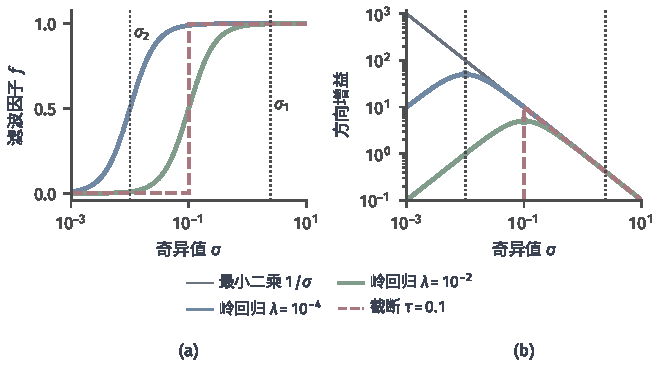
\includegraphics[width=112mm]{figures/01-basic-mathematics/03-vectors-matrices-and-multivariate-functions/matplotlib/c5-ridge-tsvd-filter-factors/figure.pdf}
 \caption{岭回归与截断SVD沿奇异方向的作用。(a)滤波因子：岭回归$f=\sigma^2/(\sigma^2+\lambda)$在$\sigma=\sqrt\lambda$处取$1/2$并连续过渡，截断SVD在阈值$\tau$处由$0$跳到$1$。(b)方向增益：最小二乘为$1/\sigma$，岭回归为$\sigma/(\sigma^2+\lambda)$，圆点是峰值$1/(2\sqrt\lambda)$；截断后小于$\tau$的方向增益为零。竖虚线是示例~\ref{ex:ls-tsvd-steps}中矩阵的两个奇异值。}
 \label{fig:ls-ridge-tsvd-filter-factors}
\end{figure}

\subsubsection{算法实现}
先区分两件事。第~\ref{sec:ls-qr-method}节的正交算法改善的是同一问题的计算过程；正则化则主动修改了问题，以控制敏感性。修改后的问题是增广最小二乘~\eqref{eq:ls-augmented-system}，所以首选的计算路线是对增广矩阵作QR分解，它适用于任意$\bm\Gamma$。下面写出这条路线的变量、输入与预处理和计算步骤，并在主要思想的小例子上执行。

\begin{example}[增广QR求岭回归]
\label{ex:ls-ridge-augmented-qr}
本例取主要思想中的教学例：
\[
 \bm A=\begin{bmatrix}3&0\\0&1\end{bmatrix},\qquad
 \bm b=\begin{bmatrix}3\\1\end{bmatrix},\qquad
 \bm\Gamma=\bm I,\qquad \lambda=1 .
\]
无惩罚时方程相容，解为$(1,1)^\top$。下面的逐步执行都在这个例子上进行。
\end{example}

\paragraph{变量}
\begin{itemize}
 \item $\tilde{\bm A}\in\mathbb R^{(m+p)\times d}$、$\tilde{\bm b}\in\mathbb R^{m+p}$：增广矩阵与增广右端。
 \item $\bm Q\in\mathbb R^{(m+p)\times d}$、$\bm R\in\mathbb R^{d\times d}$：$\tilde{\bm A}$的经济型QR因子，$\bm Q$的列标准正交，$\bm R$为对角元为正的上三角矩阵。
 \item $\bm g\in\mathbb R^d$：变换后的右端$\bm Q^\top\tilde{\bm b}$。
 \item $\bm x\in\mathbb R^d$：正则化解$\bm x_\lambda$。
 \item $\bm r\in\mathbb R^m$：原残差$\bm b-\bm A\bm x$；另报告惩罚量$\lVert\bm\Gamma\bm x\rVert_2$。
\end{itemize}

\paragraph{输入与预处理}
输入$\bm A,\bm b,\bm\Gamma,\lambda$。先核对$\bm A$与$\bm\Gamma$的列数相同、$\bm b$的长度等于$\bm A$的行数，再把增广矩阵与增广右端构造为
\[
 \tilde{\bm A}=\begin{bmatrix}\bm A\\ \sqrt\lambda\,\bm\Gamma\end{bmatrix},\qquad
 \tilde{\bm b}=\begin{bmatrix}\bm b\\ \bm0\end{bmatrix}.
\]
例中
\[
 \tilde{\bm A}=\begin{bmatrix}3&0\\0&1\\1&0\\0&1\end{bmatrix},\qquad
 \tilde{\bm b}=\begin{bmatrix}3\\1\\0\\0\end{bmatrix}.
\]

下面的步骤要求$\tilde{\bm A}$满列秩，即条件~\eqref{eq:linear-algebra-tikhonov-common-nullspace}成立；岭回归总满足这一条件。若条件不成立，增广问题的解不唯一，要先按第~\ref{chap:linear-solution-selection}章的准则另选代表，例如对$\tilde{\bm A}$作SVD取最小范数解。

\paragraph{计算步骤}
\begin{enumerate}
 \item \textbf{QR分解。}对$\tilde{\bm A}$作Householder QR（第~\ref{sec:ls-householder}节），得到
 \[
  \tilde{\bm A}=\bm Q\bm R .
 \]
 例中$\tilde{\bm A}$的两列$(3,0,1,0)^\top$与$(0,1,0,1)^\top$已经正交，长度分别为$\sqrt{10}$与$\sqrt2$，所以分解只需把两列单位化：
 \[
  \bm Q=\begin{bmatrix}3/\sqrt{10}&0\\0&1/\sqrt2\\1/\sqrt{10}&0\\0&1/\sqrt2\end{bmatrix},\qquad
  \bm R=\begin{bmatrix}\sqrt{10}&0\\0&\sqrt2\end{bmatrix}.
 \]

 \item \textbf{变换右端。}计算
 \[
  \bm g=\bm Q^\top\tilde{\bm b} .
 \]
 例中
 \[
  \bm g=\begin{bmatrix}9/\sqrt{10}\\1/\sqrt2\end{bmatrix}.
 \]

 \item \textbf{回代。}解上三角方程
 \[
  \bm R\bm x=\bm g .
 \]
 例中$\bm R$是对角的，两个分量分别为
 \[
  x_1=\frac{9/\sqrt{10}}{\sqrt{10}}=\frac9{10},\qquad
  x_2=\frac{1/\sqrt2}{\sqrt2}=\frac12 .
 \]

 \item \textbf{核验。}回到正则化目标，计算原残差与惩罚量，并检查增广正规残差
 \[
  \bm A^\top(\bm b-\bm A\bm x)-\lambda\bm\Gamma^\top\bm\Gamma\bm x
 \]
 接近零。例中
 \[
  \bm r=\bm b-\bm A\bm x=\begin{bmatrix}3-27/10\\1-1/2\end{bmatrix}=\begin{bmatrix}3/10\\1/2\end{bmatrix},
 \]
 惩罚量为
 \[
  \lVert\bm\Gamma\bm x\rVert_2=\sqrt{\frac{81}{100}+\frac14}\approx1.030 ,
 \]
 而
 \[
  \bm A^\top\bm r-\lambda\bm x=\begin{bmatrix}9/10-9/10\\1/2-1/2\end{bmatrix}=\bm0 ,
 \]
 增广正规条件成立。
\end{enumerate}

最终得到正则化解
\[
 \bm x_\lambda=\begin{bmatrix}9/10\\1/2\end{bmatrix},
\]
与主要思想中按滤波因子逐个方向算出的结果一致。原方程本来有精确解$(1,1)^\top$，算法得到的却是$(9/10,1/2)^\top$，残差不为零。这不是计算误差，而是新目标的解：惩罚项改变了要解的问题。

\paragraph{SVD路线}
$\bm\Gamma=\bm I$时还可以直接按式~\eqref{eq:matrix-analysis-ridge-filter-factor}计算。先作一次SVD，算出$c_i=\bm u_i^\top\bm b$；此后对每个$\lambda$，只需令
\[
 z_i=\frac{\sigma_ic_i}{\sigma_i^2+\lambda}\quad(i\leq r),\qquad \bm x_\lambda=\sum_{i=1}^rz_i\bm v_i .
\]
分解与$\lambda$无关，换一个参数只需重算$r$个系数与一次组合，所以要扫描多个参数时这条路线最省。

例中改取$\lambda=9$，滤波因子变为
\[
 f_1=\frac9{9+9}=\frac12,\qquad f_2=\frac1{1+9}=\frac1{10},
\]
立即得到$\bm x_\lambda=(1/2,1/10)^\top$，不必重新分解。

\paragraph{Cholesky路线}
也可以直接解定理~\ref{thm:ls-tikhonov-existence-uniqueness}中的方程：对$\bm A^\top\bm A+\lambda\bm\Gamma^\top\bm\Gamma$作Cholesky分解（第~\ref{sec:ls-cholesky}节），再依次前代、回代。推导中的这个正规矩阵并不是必须显式形成的对象；形成它会使条件数平方，下面的算法分析说明这条路线何时可靠。

\begin{example}[直线拟合的岭回归]
\label{ex:ls-ridge-line-fit}
沿用示例~\ref{ex:ls-line-least-squares}的直线拟合数据：
\[
 \bm A=\begin{bmatrix}1&0\\1&1\\1&2\end{bmatrix},\qquad
 \bm b=\begin{bmatrix}1\\2\\2\end{bmatrix},
\]
取$\bm\Gamma=\bm I$，$\lambda=1$，按Cholesky路线逐步计算。
\end{example}

\begin{enumerate}
 \item \textbf{形成方程。}由$\bm A^\top\bm A$加上$\lambda\bm I$与$\bm A^\top\bm b$，正则化后的方程为
 \[
  \begin{bmatrix}4&3\\3&6\end{bmatrix}\bm x=\begin{bmatrix}5\\6\end{bmatrix}.
 \]

 \item \textbf{Cholesky分解。}逐列计算
 \[
  \begin{gathered}
  l_{1,1}=\sqrt4=2,\qquad l_{2,1}=\frac32=1.5,\\
  l_{2,2}=\sqrt{6-1.5^2}=\frac{\sqrt{15}}2\approx1.9365 .
  \end{gathered}
 \]

 \item \textbf{前代。}
 \[
  y_1=\frac52=2.5,\qquad
  y_2=\frac{6-1.5\times2.5}{1.9365}=\frac{9}{2\sqrt{15}}\approx1.1619 .
 \]

 \item \textbf{回代。}
 \[
  x_2=\frac{1.1619}{1.9365}=0.6,\qquad
  x_1=\frac{2.5-1.5\times0.6}{2}=0.8 .
 \]

 \item \textbf{核验。}拟合值为$\bm A\bm x=(0.8,1.4,2.0)^\top$，残差为
 \[
  \bm r=\bm b-\bm A\bm x=\begin{bmatrix}0.2\\0.6\\0\end{bmatrix},\qquad
  \bm A^\top\bm r=\begin{bmatrix}0.8\\0.6\end{bmatrix}=\lambda\bm x ,
 \]
 正则化的正规残差$\bm A^\top\bm r-\lambda\bm x$为零。
\end{enumerate}

最终得到
\[
 \bm x_\lambda=\begin{bmatrix}0.8\\0.6\end{bmatrix}.
\]
与最小二乘解$(7/6,1/2)^\top$相比，残差平方由$1/6$增至$0.4$，解的长度由$1.269$降为$1$。

按SVD路线核对：$\sigma_1^2\approx7.162$，$\sigma_2^2\approx0.838$，滤波因子为$f_1\approx0.877$、$f_2\approx0.456$。$\sigma_2^2$与$\lambda$相当，第二个方向被压掉约一半。

\paragraph{大型问题}
$\bm A$很大且只能通过乘向量访问时，可以把LSQR（第~\ref{sec:ls-lsqr}节）用于增广问题~\eqref{eq:ls-augmented-system}：$\tilde{\bm A}$乘向量只需分别乘$\bm A$与$\bm\Gamma$，不必形成增广矩阵。

\subsubsection{算法分析}

\paragraph{正确性}
由定理~\ref{thm:ls-tikhonov-existence-uniqueness}，正则化目标的极小点就是增广问题~\eqref{eq:ls-augmented-system}的最小二乘解。条件~\eqref{eq:linear-algebra-tikhonov-common-nullspace}成立时$\tilde{\bm A}$满列秩，$\bm R$可逆，增广QR回代得到的就是这个唯一解；三条路线解的是同一个问题，在精确算术下给出同一个$\bm x_\lambda$。

\paragraph{数值敏感度}
增广QR对$\tilde{\bm A}$作正交变换，误差由$\kappa_2(\tilde{\bm A})$控制；Cholesky路线分解的是$\tilde{\bm A}^\top\tilde{\bm A}$，条件数是$\kappa_2(\tilde{\bm A})^2$。岭回归中$\tilde{\bm A}^\top\tilde{\bm A}$的特征值为$\sigma_i^2+\lambda$，所以
\begin{equation}
 \kappa_2(\tilde{\bm A})=\Bigl(\frac{\sigma_1^2+\lambda}{\sigma_d^2+\lambda}\Bigr)^{1/2}\leq\Bigl(1+\frac{\sigma_1^2}{\lambda}\Bigr)^{1/2},
 \label{eq:ls-ridge-augmented-condition}
\end{equation}
其中$\sigma_d$为第$d$个奇异值，秩亏时为零。这个界不依赖最小奇异值，即使$\bm A$秩亏也有界。所以只在$\lambda$不太小、$(1+\sigma_1^2/\lambda)u\ll1$时，Cholesky路线与增广QR同样可靠。

直线拟合例中$\kappa_2(\bm A)^2\approx8.55$，正则化后$\kappa_2(\tilde{\bm A})^2\approx4.44$：惩罚本身就改善了条件。

\paragraph{结果检验}
无论哪条路线，结果都要回到正则化目标核验：分别报告拟合误差$\lVert\bm A\bm x_\lambda-\bm b\rVert_2$与惩罚大小$\lVert\bm\Gamma\bm x_\lambda\rVert_2$，正规残差应检查$\bm A^\top(\bm b-\bm A\bm x_\lambda)-\lambda\bm\Gamma^\top\bm\Gamma\bm x_\lambda$，而不是原问题的$\bm A^\top\bm r$。

增广QR例中两者分别约为$0.583$与$1.030$；那里$\bm A^\top\bm r=(9/10,1/2)^\top$并不为零，用原问题的标准检查会误判为没有收敛。

\paragraph{计算代价}
增广QR处理$(m+p)\times d$的矩阵，稠密时代价为$O((m+p)d^2)$。Cholesky路线形成正规矩阵约需$md^2$次运算，分解约需$d^3/3$次，与第~\ref{sec:ls-normal-equations-method}节正规方程法的代价相同。SVD路线的一次分解为$O(md^2)$，此后每个新的$\lambda$只需$O(rd)$次运算。

\subsection{谱截断正则化}
\label{sec:ls-tsvd-solve}

\subsubsection{主要思想}

\paragraph{最小范数解中的放大}
从第~\ref{chap:singular-value-decomposition}章的SVD出发，先在奇异坐标中写出最小范数最小二乘解：
\[
 \bm A^\dagger\bm b=\sum_{i=1}^r\frac{c_i}{\sigma_i}\,\bm v_i ,\qquad c_i=\bm u_i^\top\bm b .
\]
右端在第$i$个左奇异方向上的误差进入$c_i$，再被放大$1/\sigma_i$倍。若误差预算表明某些方向的观测分量$c_i$主要是噪声，就不应在这些方向上反演。谱截断正则化因此只在可靠的奇异方向上恢复系数。

\paragraph{只保留可靠方向}
给定阈值$\tau$，取保留集$J=\{i:\sigma_i>\tau\}$；也可以事先指定保留最大的$k$个正奇异值。奇异值按降序排列，所以$J=\{1,\ldots,k\}$，$k=|J|$。令
\begin{equation}
 \bm x_k=\sum_{i=1}^k\frac{c_i}{\sigma_i}\,\bm v_i ,\qquad 1\leq k\leq r .
 \label{eq:ls-tsvd-solution}
\end{equation}
这种做法称为\term{截断SVD}（truncated SVD）求解。与岭回归的式~\eqref{eq:matrix-analysis-ridge-filter-factor}对照，它相当于把滤波因子取为$f_i=1$（$i\leq k$）或$f_i=0$（$i>k$）。

\begin{example}[对角矩阵的谱截断]
\label{ex:ls-tsvd-diagonal}
取$\bm A=\operatorname{diag}(1,1/100)$，真实系数$\bm x_{\mathrm{true}}=(1,1)^\top$，无噪声的观测为$(1,1/100)^\top$。设第二个观测带误差$2/100$，实际得到
\[
 \bm b=\begin{bmatrix}1\\3/100\end{bmatrix}.
\]
这里$\sigma_1=1$，$\sigma_2=1/100$，奇异向量就是坐标向量，$c_1=1$，$c_2=3/100$。按分量写出不截断时的系数、取$\tau=1/10$时的滤波因子与截断后的系数：
\[
 \begin{aligned}
 &\text{第一个方向：}&& \frac{c_1}{\sigma_1}=1,\qquad f_1=1,\qquad f_1\frac{c_1}{\sigma_1}=1;\\
 &\text{第二个方向：}&& \frac{c_2}{\sigma_2}=3,\qquad f_2=0,\qquad f_2\frac{c_2}{\sigma_2}=0 .
 \end{aligned}
\]
不截断时得到$(1,3)^\top$：第二个方向把误差$2/100$放大了一百倍。截断只保留$\sigma_1$，得到
\[
 \bm x_1=\begin{bmatrix}1\\0\end{bmatrix}.
\]

两种恢复的误差范数分别为
\[
 \lVert(1,3)^\top-(1,1)^\top\rVert_2=2,\qquad \lVert(1,0)^\top-(1,1)^\top\rVert_2=1,
\]
截断的误差较小。

但这个改善是以丢掉真实的第二分量为代价的：若真值的第二分量很大而噪声很小，截断反而更差。不能从一个算例推断任意真值和噪声下截断都更好，算法分析中的误差分解说明了一般情形。
\end{example}

\paragraph{限制子空间上的最小二乘}
截断解并非随意拼出的近似，它是一个限制在子空间上的最小二乘解。把系数限制在$\operatorname{span}\{\bm v_1,\ldots,\bm v_k\}$中，写$\bm x=\sum_{i\leq k}z_i\bm v_i$，则$\bm A\bm x=\sum_{i\leq k}\sigma_iz_i\bm u_i$。把$\bm b$按左奇异方向与列空间的正交补分开，残差平方分成三部分：
\begin{equation}
 \begin{aligned}
 \lVert\bm A\bm x-\bm b\rVert_2^2
 &=\sum_{i=1}^k(\sigma_iz_i-c_i)^2+\sum_{i=k+1}^rc_i^2\\
 &\quad+\lVert(\bm I-\bm A\bm A^\dagger)\bm b\rVert_2^2 .
 \end{aligned}
 \label{eq:ls-tsvd-restricted-residual}
\end{equation}
只有第一项依赖$\bm z$，取$z_i=c_i/\sigma_i$使它为零，就得到$\bm x_k$。被舍弃方向上的观测分量$c_{k+1},\ldots,c_r$无法再被拟合，全部转入残差。对角例中残差为
\[
 \bm b-\bm A\bm x_1=\begin{bmatrix}0\\3/100\end{bmatrix},
\]
正是被舍弃的观测分量$c_2$。

\paragraph{与截断矩阵的关系}
用矩阵写，令
\begin{equation}
 \bm A_k=\sum_{i=1}^k\sigma_i\bm u_i\bm v_i^\top ,
 \label{eq:ls-truncated-matrix}
\end{equation}
即只保留前$k$项的SVD，则$\bm x_k=\bm A_k^\dagger\bm b$，是以$\bm A_k$代替$\bm A$后的最小范数最小二乘解。第~\ref{chap:matrix-approximation}章将把$\bm A_k$作为矩阵的低秩逼近来研究。两者共用同一个分解，目的却不同：低秩逼近要重建矩阵，截断求解要从带误差的观测中稳定地恢复输入。

\subsubsection{算法实现}
算法先求SVD并把右端投影到左奇异方向，再按保留规则逐个方向设置系数，最后合成解并读出残差。下面写出计算中用到的变量、输入与预处理和计算步骤，并在一个近共线的设计上执行。

\begin{example}[近共线设计的截断求解]
\label{ex:ls-tsvd-steps}
设计矩阵与观测为
\[
 \bm A=\begin{bmatrix}1&1\\1&1.01\\1&0.99\end{bmatrix},\qquad
 \bm b=\begin{bmatrix}1\\1.1\\0.9\end{bmatrix}.
\]
这是示例~\ref{ex:ls-nearly-collinear-design}中取$\bm c=(1,1,1)^\top$、$\bm q=(0,1,-1)^\top$、$\varepsilon=0.01$、$\delta=0.1$的情形。阈值取$\tau=0.1$。
\end{example}

\paragraph{变量}
\begin{itemize}
 \item $\sigma_i,\bm u_i,\bm v_i$（$i\leq r$）：经济型SVD的正奇异值与奇异向量，奇异值按降序排列。
 \item $\bm c\in\mathbb R^r$：右端在左奇异方向上的分量$c_i=\bm u_i^\top\bm b$。
 \item $J$与$k=|J|$：保留集与保留的方向数。
 \item $\bm z\in\mathbb R^r$：解在右奇异方向上的系数。
 \item $\bm x\in\mathbb R^d$：截断解$\bm x_k$。
 \item $\bm r\in\mathbb R^m$：原残差$\bm b-\bm A\bm x$。
\end{itemize}

\paragraph{输入与预处理}
输入$\bm A,\bm b$与阈值$\tau$（或保留数$k$），求$\bm A$的经济型SVD。例中
\[
 \sigma_1\approx2.4495,\qquad \sigma_2\approx0.0100,
\]
右奇异向量为
\[
 \bm v_1\approx\frac1{\sqrt2}\begin{bmatrix}1\\1\end{bmatrix},\qquad
 \bm v_2\approx\frac1{\sqrt2}\begin{bmatrix}1\\-1\end{bmatrix},
\]
左奇异向量为
\[
 \bm u_1\approx\begin{bmatrix}0.5773\\0.5802\\0.5745\end{bmatrix},\qquad
 \bm u_2\approx\begin{bmatrix}0.0024\\-0.7047\\0.7095\end{bmatrix}.
\]

\paragraph{计算步骤}
\begin{enumerate}
 \item \textbf{投影右端。}计算
 \[
  \bm c=\bm U^\top\bm b .
 \]
 例中
 \[
  c_1\approx1.7326,\qquad c_2\approx-0.1343 .
 \]

 \item \textbf{确定保留集。}取$J=\{i:\sigma_i>\tau\}$，$k=|J|$。例中只有$\sigma_1$超过阈值$0.1$，所以
 \[
  J=\{1\},\qquad k=1 .
 \]

 \item \textbf{设置系数。}逐项令
 \begin{equation}
  z_i=\begin{cases}c_i/\sigma_i,& i\in J,\\ 0,& i\notin J .\end{cases}
  \label{eq:ls-tsvd-coefficients}
 \end{equation}
 所有除法只在保留的正奇异值上执行。例中
 \[
  z_1=\frac{1.7326}{2.4495}\approx0.7073,\qquad z_2=0 .
 \]
 若不截断，第二个系数将是$c_2/\sigma_2\approx-13.435$。

 \item \textbf{合成解。}计算
 \[
  \bm x=\sum_{i\in J}z_i\bm v_i .
 \]
 例中
 \[
  \bm x_1\approx0.7073\,\bm v_1\approx\begin{bmatrix}0.5001\\0.5002\end{bmatrix}.
 \]

 \item \textbf{读出拟合值与残差。}由$\bm A\bm v_i=\sigma_i\bm u_i$，拟合值是
 \begin{equation}
  \bm A\bm x_k=\sum_{i\in J}c_i\bm u_i ,
  \label{eq:ls-tsvd-fitted-values}
 \end{equation}
 不必再乘$\bm A$。残差由被舍弃方向的分量与列空间外的部分组成。例中$\bm b$在$\bm A$的列空间内（$\lVert\bm b\rVert_2^2=c_1^2+c_2^2$），残差全部来自被舍弃的第二个方向：
 \[
  \bm r=c_2\bm u_2\approx\begin{bmatrix}-0.0003\\0.0947\\-0.0953\end{bmatrix},\qquad
  \lVert\bm r\rVert_2=|c_2|\approx0.1343 .
 \]

 \item \textbf{核验。}检查原残差，并检查限制子空间中的正规条件
 \begin{equation}
  \bm v_i^\top\bm A^\top\bm r=0\qquad(i\in J).
  \label{eq:ls-tsvd-restricted-normal-condition}
 \end{equation}
 例中$\bm v_1^\top\bm A^\top\bm r=\sigma_1\bm u_1^\top\bm r=0$成立；完整的正规残差却是
 \[
  \bm A^\top\bm r=\sigma_2c_2\bm v_2\approx\begin{bmatrix}-0.00095\\0.00095\end{bmatrix},
 \]
 长度约为$0.0013$，不为零：$\bm x_1$不是原问题的最小二乘解。
\end{enumerate}

最终得到截断解
\[
 \bm x_1\approx\begin{bmatrix}0.50\\0.50\end{bmatrix}.
\]
换一个阈值只需增减和式中的项。若取$\tau<\sigma_2$，第二个方向贡献$(c_2/\sigma_2)\bm v_2\approx-13.4\,\bm v_2$，解变为精确拟合的$(-9,10)^\top$，与示例~\ref{ex:ls-nearly-collinear-design}的最小二乘解相同。

两者对照，截断以约$0.134$的残差为代价，把一对此增彼减的大系数换成了两个接近$0.5$的系数。

\subsubsection{算法分析}

\paragraph{误差分解}
设观测由真实输入加噪声得到。截断解的误差与拟合损失都可以按奇异方向分开。

\begin{theorem}[截断SVD的误差分解]
\label{thm:ls-tsvd-error-decomposition}
设$\bm b=\bm A\bm x_{\mathrm{true}}+\bm e$，$\bm x_{\mathrm{true}}\in\operatorname{range}\bm A^\top$，$1\leq k\leq r$。则
\begin{equation}
 \begin{aligned}
 \bm x_k-\bm x_{\mathrm{true}}
 &=\sum_{i=1}^k\frac{\bm u_i^\top\bm e}{\sigma_i}\,\bm v_i\\
 &\quad-\sum_{i=k+1}^r(\bm v_i^\top\bm x_{\mathrm{true}})\,\bm v_i ,
 \end{aligned}
 \label{eq:ls-tsvd-error-decomposition}
\end{equation}
两项正交，第一项的长度不超过$\lVert\bm e\rVert_2/\sigma_k$。此外
\begin{equation}
 \begin{gathered}
 \lVert\bm b-\bm A\bm x_k\rVert_2^2=\lVert\bm b-\bm A\hat{\bm x}\rVert_2^2+\sum_{i=k+1}^rc_i^2,\\
 \bm A^\top(\bm b-\bm A\bm x_k)=\sum_{i=k+1}^r\sigma_ic_i\bm v_i ,
 \end{gathered}
 \label{eq:ls-tsvd-residual-decomposition}
\end{equation}
其中$\hat{\bm x}$为任一最小二乘解。
\end{theorem}
\begin{proof}
由$c_i=\sigma_i\bm v_i^\top\bm x_{\mathrm{true}}+\bm u_i^\top\bm e$，
\[
 \bm x_k=\sum_{i\leq k}\Bigl(\bm v_i^\top\bm x_{\mathrm{true}}+\frac{\bm u_i^\top\bm e}{\sigma_i}\Bigr)\bm v_i .
\]
而$\bm x_{\mathrm{true}}=\sum_{i\leq r}(\bm v_i^\top\bm x_{\mathrm{true}})\bm v_i$，相减即得误差式。两项落在互相正交的$\bm v_i$上；第一项长度的平方为
\[
 \sum_{i\leq k}\frac{(\bm u_i^\top\bm e)^2}{\sigma_i^2}\leq\frac{\lVert\bm e\rVert_2^2}{\sigma_k^2}.
\]

再看残差。由$\bm A\bm x_k=\sum_{i\leq k}c_i\bm u_i$，
\[
 \bm b-\bm A\bm x_k=(\bm I-\bm A\bm A^\dagger)\bm b+\sum_{i>k}c_i\bm u_i ,
\]
两部分正交，前者就是最小二乘残差；再用$\bm A^\top\bm u_i=\sigma_i\bm v_i$与$\bm A^\top(\bm I-\bm A\bm A^\dagger)=\bm0$得正规残差。
\end{proof}

第一项是保留方向的噪声放大，它的界由$\sigma_k$而不是$\sigma_r$决定；第二项是舍弃方向上真实输入的全部损失，这就是截断引入的偏差。在例~\ref{ex:ls-tsvd-diagonal}中，不截断（$k=r$）时没有舍弃项，误差$(0,2)^\top$全部是噪声放大；截断后误差$(0,-1)^\top$全部是偏差。

拟合的代价是残差平方多出被舍弃的$c_i^2$。正规残差只落在被舍弃的方向上，所以限制子空间中的正规条件成立，而完整的正规条件一般不成立；近共线例中正规残差$\sigma_2c_2\bm v_2$的长度约为$0.0013$，正是这一项。

\paragraph{计算代价}
主要计算代价是一次SVD，稠密时为$O(md^2)$量级。分解完成后，投影右端约需$mr$次运算，合成解约需$dk$次；换阈值或换保留数不必重新分解。

\subsubsection{与岭回归的比较}
岭回归连续地压低小奇异值方向，截断则把滤波因子直接取成$1$（$i\leq k$）或$0$（$i>k$），两者在图~\ref{fig:ls-ridge-tsvd-filter-factors}中分别是光滑曲线与阶梯。要看出这种差别对结果的影响，最直接的办法是在同一组数据上比较两者的解、残差，以及观测改动后解的变化。

\begin{example}[岭回归与截断SVD的比较]
\label{ex:ls-regularization-response}
沿用示例~\ref{ex:ls-tsvd-steps}的数据，再把$\bm b$改为$(1,1.11,0.89)^\top$，这个扰动几乎全部落在$\bm u_2$上。下表前两列是原观测下各方法的解与残差长度，最后一列是改动观测后系数的变化与观测的变化之比：
\[
 \begin{array}{lccc}
  \text{方法} & \bm x & \lVert\bm r\rVert_2 & \lVert\Delta\bm x\rVert_2/\lVert\Delta\bm b\rVert_2\\[2pt]
  \text{最小二乘} & (-9,\,10)^\top & 0 & 100\\
  \lambda=10^{-4} & (-4.25,\,5.25)^\top & 0.067 & 50\\
  \lambda=10^{-2} & (0.41,\,0.59)^\top & 0.133 & 0.99\\
  k=1 & (0.50,\,0.50)^\top & 0.134 & 0.002
 \end{array}
\]
响应比就是第二个方向的增益：最小二乘为$1/\sigma_2=100$，岭回归为$\sigma_2/(\sigma_2^2+\lambda)$，截断后为零，剩下的$0.002$来自扰动在$\bm u_1$上的微小分量。
\end{example}

表中可以读出两点。第一，精确拟合的大系数全部来自第二个方向，系数越稳定，残差越大。第二，$\lambda=10^{-2}$的岭回归与$k=1$的截断已经很接近：这时$f_2\approx0.0099$，岭回归几乎也把第二个方向舍去了。

两种方法适用的场景不同。奇异值在某处明显下降时，截断位置有自然的选择，截断把可信与不可信的方向分得最清楚；奇异值缓慢衰减、没有明显间隔时，连续衰减的岭回归更平稳。

阈值应联系噪声规模、截断处的奇异值间隔和任务目标。取$\tau$为数据误差的估计，就是只在第~\ref{sec:ls-pseudoinverse-rank-change}节意义下可辨认的方向上反演；它不等同于按机器精度判定精确秩，只有数据仅含舍入误差时两者才一致。

\subsubsection{与低秩逼近的边界}
截断求解与矩阵的低秩逼近共用$\bm A_k$，但两者的最优性不能互相借用。第~\ref{chap:matrix-approximation}章将证明，$\bm A_k$在谱范数与Frobenius范数下是最佳秩$k$重建（定理~\ref{thm:matrix-analysis-best-low-rank}）。这一结论只说$\bm A_k$离$\bm A$最近，不说$\bm x_k$拟合得最好：由定理~\ref{thm:ls-tsvd-error-decomposition}的正规残差，除非被舍弃的$c_i$全为零，$\bm x_k$不是原问题的最小二乘解。矩阵逼近的最优性也不涉及$\bm x_{\mathrm{true}}$与$\bm e$，更不能由它断言$\bm x_k$最接近未知的真实输入。

所以截断求解要同时说明保留了哪些方向、噪声水平多大、允许多大的拟合损失。保留的方向本身是否可靠，还要看截断处的间隔$\sigma_k-\sigma_{k+1}$：间隔很小时，扰动可能使前$k$个奇异方向明显偏转，第~\ref{sec:ls-subspace-sensitivity}节的奇异值与子空间扰动界可以用来判断。

\section{求解方法的比较与选择}
\label{sec:ls-method-selection}

第~\ref{chap:direct-linear-solvers}—\ref{chap:row-projection-methods}章分别给出了直接分解、最小二乘的直接求解、定常迭代、Krylov子空间法与行列投影法。每一章都在自己的前提下说明了方法怎样计算、何时成立，但没有把不同章的方法放在同一个问题上比较。本节做这件事。

比较之前，先要确定比较什么。同一个矩阵上，两种方法可能求的根本不是同一个解；即使求同一个解，一种方法也可能要求另一种方法不需要的矩阵性质。所以本节按四个维度依次比较，每个维度回答一个问题。

第一个维度是求解目标：要的是精确解、最小二乘解还是最小范数解，以及方法能否直接面对这个目标。第二个维度是矩阵条件：方法对矩阵的形状、对称性、正定性和秩有什么要求，需要怎样访问矩阵。第三个维度是计算开销与收敛速度：达到同一精度一共要付出多少运算、存储和数据读取。第四个维度是数值稳定性：有限精度下结果的误差来自哪里，算法本身会不会额外放大误差。最后把四个维度合起来，给出几类典型问题的取舍。

比较的对象始终是“达到相同要求的总成本”。第~\ref{sec:ls-truncated-svd-ridge}节的正则化与谱截断不在此列：它们改变了求解目标，得到的系数较小、计算也可能更便宜，但这不表示把原问题解得更准确，不能与求原问题的方法按成本或误差直接比较。

\subsection{求解目标与方法适用性}
\label{sec:ls-method-selection-goals}

\paragraph{三种验收要求}
第~\ref{chap:linear-solution-selection}章区分了三种求解目标。它们在多数情况下不同，因此检验一个结果是否合格的标准也不同。

相容方程$\bm A\bm x=\bm b$要求原残差为零；一般最小二乘问题$\min_{\bm x}\lVert\bm A\bm x-\bm b\rVert_2$只要求残差与列空间正交；最小范数解在此之上还要求解不含$\ker\bm A$的分量（第~\ref{sec:ls-select-among-solutions}节）。记$\bm r=\bm b-\bm A\bm x$，三种要求依次为
\begin{equation}
 \bm r=\bm0;\qquad
 \bm A^\top\bm r=\bm0;\qquad
 \bm A^\top\bm r=\bm0\ \text{且}\ \bm x\in\operatorname{range}\bm A^\top .
 \label{eq:ls-method-selection-acceptance}
\end{equation}

方程相容时，前两种要求给出同一个解集。方程不相容时，最优残差停在一个正的长度上，第一种要求无法满足。以第~\ref{sec:ls-lsqr}节的不相容系统为例：
\[
 \bm A=\begin{bmatrix}1&0\\0&2\\0&0\end{bmatrix},\qquad
 \bm b=\begin{bmatrix}1\\1\\1\end{bmatrix}.
\]
它的最小二乘解与最优残差为
\[
 \hat{\bm x}=\begin{bmatrix}1\\1/2\end{bmatrix},\qquad
 \hat{\bm r}=\begin{bmatrix}0\\0\\1\end{bmatrix}.
\]
这里$\lVert\hat{\bm r}\rVert_2=1$，而$\bm A^\top\hat{\bm r}=\bm0$，$\hat{\bm x}$已经是最小二乘解。若按原残差趋于零来判断，任何方法在这个问题上都不会“成功”。所以不能把所有算法都按$\lVert\bm r\rVert_2\to0$检验。

第三种要求在解不唯一时才起作用。例~\ref{ex:ls-qr-min-norm-run}的方程为
\[
 \begin{bmatrix}1&0&1\\0&1&1\end{bmatrix}\bm x=\begin{bmatrix}1\\2\end{bmatrix}.
\]
它有无穷多解，$(0,1,1)^\top$与$(1,2,0)^\top$的残差都为零，但前者与$\ker\bm A$的方向$(1,1,-1)^\top$正交，范数为$\sqrt2$；后者含零空间分量，范数为$\sqrt5$。残差检验分不出两者，只有第三种要求能把最小范数解挑出来。

\paragraph{经正规方程转换}
求解目标与方法要求的输入不一致时，可以先改写问题。最常见的改写是正规方程。满列秩时，最小二乘解是
\[
 \bm A^\top\bm A\bm x=\bm A^\top\bm b
\]
的唯一解，系数矩阵$\bm A^\top\bm A$对称正定。于是长方的最小二乘问题变成一个对称正定方程，可以交给Cholesky分解、CG或在对称正定矩阵上收敛的定常迭代。

这种改写有三项代价。其一，显式形成$\bm A^\top\bm A$时，稀疏矩阵可能变稠密：$\bm A$只要有一行全是非零元，这一行的外积就填满整个Gram矩阵。

其二，条件数变为平方（式~\eqref{eq:matrix-analysis-normal-equation-condition-square}），
\[
 \kappa_2(\bm A^\top\bm A)=\kappa_2(\bm A)^2 .
\]
例~\ref{ex:ls-rhs-perturbation-near-parallel}的$\bm A_2$取$\varepsilon=10^{-8}$时，$\kappa_2(\bm A_2)\approx2\times10^8$，双精度下两列仍可区分；但Gram矩阵的元素$1+\varepsilon^2$舍入后就是$1$，存下来的$\bm A_2^\top\bm A_2$已经奇异（第~\ref{sec:ls-ls-regularization-sensitivity}节）。

其三，不显式形成$\bm A^\top\bm A$时，迭代法每次作用它仍要一次$\bm A$乘向量和一次$\bm A^\top$乘向量。此外，秩亏时$\bm A^\top\bm A$只是半正定，正定矩阵上的唯一性与收敛保证都不能照搬。

\paragraph{经增广方程转换}
另一种改写不消去残差，而把它也当作未知量：残差的定义$\bm r+\bm A\bm x=\bm b$与正交条件$\bm A^\top\bm r=\bm0$合起来，是一个关于$(\bm r,\bm x)$的方阵方程。下面的定理说明这个方程的性质，它决定了能用哪些方法求解。

\begin{theorem}[最小二乘的增广方程]
\label{thm:ls-augmented-kkt-system}
设$\bm A\in\mathbb R^{m\times d}$满列秩，则方程
\begin{equation}
 \begin{bmatrix}\bm I_m&\bm A\\ \bm A^\top&\bm0\end{bmatrix}
 \begin{bmatrix}\bm r\\ \bm x\end{bmatrix}
 =\begin{bmatrix}\bm b\\ \bm0\end{bmatrix}
 \label{eq:ls-augmented-kkt-system}
\end{equation}
有唯一解，$\bm x$为最小二乘解，$\bm r$为相应残差；其系数矩阵对称、可逆且不定。
\end{theorem}
\begin{proof}
第一块行给出$\bm r=\bm b-\bm A\bm x$，第二块行就是正规方程$\bm A^\top(\bm b-\bm A\bm x)=\bm0$，所以解与最小二乘解一一对应。对称性显然。

若系数矩阵作用于$(\bm r;\bm x)$得零，则$\bm r=-\bm A\bm x$且$\bm A^\top\bm A\bm x=\bm0$，满列秩时只能$\bm x=\bm0$、$\bm r=\bm0$，故可逆。

再看不定性。取$(\bm u;\bm0)$，$\bm u\ne\bm0$，二次型为$\lVert\bm u\rVert_2^2>0$；取$(-\bm A\bm x;\bm x)$，$\bm x\ne\bm0$，二次型为$-\lVert\bm A\bm x\rVert_2^2<0$，故不定。
\end{proof}

在上面的不相容例子中，$\bm A$的两列分别只在第一、二行非零。按$(r_1,x_1)$、$(r_2,x_2)$、$r_3$重排未知量后，$5$阶增广矩阵分解为三个对角块：
\[
 \begin{bmatrix}1&1\\1&0\end{bmatrix},\qquad
 \begin{bmatrix}1&2\\2&0\end{bmatrix},\qquad
 \begin{bmatrix}1\end{bmatrix}.
\]
二阶块$\left[\begin{smallmatrix}1&\sigma\\\sigma&0\end{smallmatrix}\right]$的特征值是$(1\pm\sqrt{1+4\sigma^2})/2$，所以增广矩阵的五个特征值约为
\[
 1.618,\quad -0.618,\quad 2.562,\quad -1.562,\quad 1,
\]
正负都有，确实不定。解出的$(\bm r;\bm x)=(0,0,1;\,1,1/2)$正是前面的最优残差与最小二乘解。

因此，满列秩最小二乘也可以用分块$\mathrm{LDL}^\top$分解（第~\ref{sec:ls-ldlt}节）或MINRES（第~\ref{sec:ls-minres}节）求解，而不能用要求正定的Cholesky或CG。与正规方程相比，这一改写保留了$\bm A$的稀疏结构，也不使条件数平方；代价是未知量从$d$个增加到$m+d$个，存储与预条件都要按新的分块结构设计。

\paragraph{三种适用方式}
有了这两种改写，方法与目标的关系可以分成三种，下文统一使用这三种说法。

“直接适用”指方法直接以原问题的目标和数据为输入，例如QR、SVD与LSQR直接处理矩形最小二乘。“需转换”指先改变方程的表示，例如经正规方程或增广方程变成方阵方程，再交给方阵方法。“需扩展版本”指要修改算法本身，才能处理秩亏、不相容或最小范数的要求，例如扩展Kaczmarz相对于标准Kaczmarz。

三种方式都只说明方法能够面对这个目标，不说明它一定收敛。能对转换后的方程写出迭代公式，并不等于转换后的矩阵满足这种迭代的收敛条件。

\subsection{矩阵条件}
\label{sec:ls-method-selection-matrix}

目标确定以后再看矩阵。每种方法的正确性与收敛性都建立在一组矩阵条件之上：形状是方阵还是长方，是否对称、正定，秩是否完全。除此之外，方法还规定了它怎样读取矩阵：有的要把矩阵存下来做分解，有的只要计算矩阵乘向量，有的还要转置乘向量，有的每次只读一行。实际问题能提供哪种访问方式，常常与矩阵的数学性质一样限制方法的选择。

下面按章分组说明，最后用表~\ref{tab:ls-method-applicability}汇总。表中的迭代法都按第~\ref{chap:stationary-iterations}—\ref{chap:row-projection-methods}章建立的基本版本比较，某一行的限制不能推广到同名算法的所有扩展。

\paragraph{方阵的直接分解}
第~\ref{chap:direct-linear-solvers}章的方法都要求矩阵非奇异，并且要能存下矩阵和因子。带部分选主元的LU分解对任何非奇异方阵都能进行。Cholesky分解要求对称正定，这一条件既是充分的也是必要的，运算量是LU的一半。分块$\mathrm{LDL}^\top$分解只要求对称非奇异，允许不定，负主元与二阶块保留在$\bm D$中。低秩更新不是独立的分解，它要求修改前的矩阵已经分解、修改的秩很低，并且辅助矩阵可逆；它节省的是重新分解的工作。

这些方法都以方阵方程为对象，用于不相容最小二乘时须先转换：Cholesky用于满列秩的正规方程，分块$\mathrm{LDL}^\top$用于增广方程。普通LU直接作用于长方矩阵时并不保留最小二乘的目标。

\paragraph{最小二乘的直接求解}
第~\ref{chap:direct-least-squares-solvers}章的三条路线直接以最小二乘为目标，区别在于对秩的要求。正规方程法要求满列秩，并承受条件数平方。QR求解在满列秩时回代得到唯一最小二乘解，在满行秩时对$\bm A^\top$分解得到最小范数解；秩亏时$\bm R$出现零对角元，基本QR不能直接给出最小范数解。SVD求解对任意形状和秩都给出$\bm A^\dagger\bm b$，代价是分解更贵，小奇异值处的误差放大也要另行处理。三条路线都需要显式存储$\bm A$；正规方程法还可以按行累计Gram矩阵，适合观测逐批到达的情形。

\paragraph{定常迭代}
第~\ref{chap:stationary-iterations}章的方法求解可逆方阵方程，收敛当且仅当迭代矩阵的谱半径小于一：
\[
 \rho(\bm I-\bm M^{-1}\bm A)<1 .
\]
各方法的区别在于有哪些条件能保证这一点。Richardson只需矩阵乘向量；对称正定时收敛当且仅当$0<\alpha<2/\lambda_{\max}$。Jacobi与Gauss--Seidel要求对角元非零，这只保证可以执行；严格行对角占优对两者都保证收敛，对称正定只保证Gauss--Seidel收敛，不保证Jacobi收敛。SOR在对称正定矩阵上收敛当且仅当$0<\omega<2$。SSOR要求对称正定与$0<\omega<2$，每轮做前向与反向两次扫掠。

定常迭代用于最小二乘时须经正规方程转换。满列秩时$\bm A^\top\bm A$对称正定，Gauss--Seidel、SOR与SSOR的收敛保证随之成立，Jacobi仍须另行检查。在贯穿例~\ref{ex:ls-stationary-running-example}的$\bm A=\left[\begin{smallmatrix}4&1\\1&3\end{smallmatrix}\right]$上，五种方法都收敛，但谱半径各不相同，这在下一小节比较。

\paragraph{Krylov子空间法}
第~\ref{chap:krylov-methods}章的求解器按矩阵类型分工。CG要求对称正定。MINRES要求对称非奇异，允许不定；用于奇异对称矩阵时，判断是否到达最小二乘解要看$\lVert\bm A\bm r_k\rVert_2$，所得的解一般也不是最小范数解。GMRES、BiCG与BiCGSTAB适用于一般非奇异方阵，不要求对称。

这几种方法对矩阵访问的要求不同。CG、MINRES、GMRES与BiCGSTAB只需计算$\bm A\bm v$；BiCG还需计算$\bm A^\top\bm u$，转置作用难以获得时就不能使用。它们都是方阵方法，用于不相容最小二乘须先转换：CG可用于满列秩的正规方程，MINRES可用于增广方程。

LSQR与LSMR是第~\ref{chap:krylov-methods}章中直接处理长方矩阵的两种迭代法。它们允许长方、秩亏和不相容，每轮需要$\bm A\bm v$与$\bm A^\top\bm u$各一次，零初值时选出最小范数解。两者也能求解相容方程。

\paragraph{行列投影法}
第~\ref{chap:row-projection-methods}章的方法每次只读一行或一列。标准Kaczmarz求解相容方程，零初值时收敛到最小范数解；方程不相容时，它在各行的解之间往返，不论循环还是随机选行，都不会停在最小二乘解上。扩展Kaczmarz用列投影逐步分离出右端中不可拟合的部分，再对校正后的相容方程作行投影，因此能求最小范数最小二乘解，代价是还要能按列访问矩阵。

\paragraph{汇总}
表~\ref{tab:ls-method-applicability}汇总了上面的条件。表中“需转换”时，要对转换后的系统重新检查结构、条件数、零空间与误差度量；标为“直接适用”也不意味着可以省去预条件、停止检验与退化处理。

\begin{BookLongTable}{@{}>{\RaggedRight\arraybackslash}p{22mm}>{\RaggedRight\arraybackslash}p{\dimexpr(\linewidth-22mm-6\tabcolsep)*2/5\relax}>{\RaggedRight\arraybackslash}p{\dimexpr(\linewidth-22mm-6\tabcolsep)*3/10\relax}>{\RaggedRight\arraybackslash}p{\dimexpr(\linewidth-22mm-6\tabcolsep)*3/10\relax}@{}}
\toprule
方法 & 对矩阵的要求 & 对矩阵的访问 & 不相容最小二乘\\
\midrule
\endfirsthead
\multicolumn{4}{@{}l}{\small 表~\thetable（续）}\\
\toprule
方法 & 对矩阵的要求 & 对矩阵的访问 & 不相容最小二乘\\
\midrule
\endhead
\midrule
\multicolumn{4}{r@{}}{\small 续下页}\\
\endfoot
\bottomrule
\caption{各方法的矩阵条件与适用方式（基本版本）。方法名后括号内为所在节。}
\label{tab:ls-method-applicability}\\
\endlastfoot
LU（\ref{sec:ls-lu}） & 非奇异方阵 & 存储并分解 & 需转换\\
Cholesky（\ref{sec:ls-cholesky}） & 对称正定 & 存储并分解 & 经正规方程，须满列秩\\
分块$\mathrm{LDL}^\top$（\ref{sec:ls-ldlt}） & 对称非奇异，可不定 & 存储并分解 & 经增广方程，须满列秩\\
低秩更新（\ref{sec:ls-woodbury}） & 原矩阵已分解，修改秩低，辅助矩阵可逆 & 旧因子与低秩因子 & 不直接适用\\
正规方程法（\ref{sec:ls-normal-equations-method}） & 满列秩 & 存储，可按行累计 & 直接适用，条件数平方\\
QR（\ref{sec:ls-qr-method}） & 满列秩或满行秩 & 存储并分解 & 直接适用\\
SVD（\ref{sec:ls-svd-solve}） & 任意形状与秩 & 存储并分解 & 直接适用，给出$\bm A^\dagger\bm b$\\
Richardson（\ref{sec:ls-richardson}） & $\rho(\bm I-\alpha\bm A)<1$ & $\bm A\bm v$ & 需转换\\
Jacobi（\ref{sec:ls-jacobi}） & 对角元非零，谱半径小于一 & 按行读取 & 需转换，须另查收敛\\
Gauss--Seidel、SOR（\ref{sec:ls-gauss-seidel}、\ref{sec:ls-sor}） & 对角元非零，谱半径小于一 & 按行顺序读取 & 经正规方程\\
SSOR（\ref{sec:ls-ssor}） & 对称正定，$0<\omega<2$ & 前后两次扫掠 & 经正规方程\\
CG（\ref{sec:ls-conjugate-gradient}） & 对称正定 & $\bm A\bm v$ & 经正规方程\\
MINRES（\ref{sec:ls-minres}） & 对称非奇异，可不定 & $\bm A\bm v$ & 经增广方程\\
GMRES（\ref{sec:ls-gmres}） & 非奇异方阵 & $\bm A\bm v$ & 需转换\\
BiCG（\ref{sec:ls-bicg}） & 非奇异方阵 & $\bm A\bm v$与$\bm A^\top\bm u$ & 需转换\\
BiCGSTAB（\ref{sec:ls-bicgstab}） & 非奇异方阵 & $\bm A\bm v$ & 需转换\\
LSQR（\ref{sec:ls-lsqr}） & 任意形状与秩 & $\bm A\bm v$与$\bm A^\top\bm u$ & 直接适用\\
LSMR（\ref{sec:ls-lsmr}） & 任意形状与秩 & $\bm A\bm v$与$\bm A^\top\bm u$ & 直接适用\\
标准Kaczmarz（\ref{sec:ls-kaczmarz}） & 相容方程 & 逐行 & 不收敛到最小二乘解\\
扩展Kaczmarz（\ref{sec:ls-extended-kaczmarz}） & 任意形状与秩 & 逐行与逐列 & 需扩展版本，即本方法\\
\end{BookLongTable}

\subsection{计算开销与收敛速度}
\label{sec:ls-method-selection-cost}

\paragraph{总成本的组成}
两种方法都能面对同一个目标时，下一个问题是哪一种更省。直观地说，一次求解的总成本是“准备工作”加上“每步工作乘步数”：
\begin{equation}
 \text{总成本}\approx\text{准备成本}+\text{步数}\times\text{每步成本}.
 \label{eq:ls-method-selection-total-cost}
\end{equation}
准备成本包括分解、形成Gram矩阵或构造预条件；每步成本包括矩阵乘向量、内积、向量更新与辅助求解；步数由收敛速度决定。此外还要计入额外存储，以及并行计算中各处理器之间交换数据的通信。直接法几乎全部成本都在准备上，步数可以看作一；迭代法准备便宜，成本主要由步数决定。

下面设$\bm A$有$q$个非零元素。一次矩阵乘向量对每个非零元做一次乘法和一次加法，约需$2q$次运算；长度为$d$的内积与向量线性组合约需与$d$同阶的运算。

\paragraph{直接法的运算量}
对稠密$d$阶方阵，LU分解约需$\tfrac23d^3$次运算，Cholesky与分块$\mathrm{LDL}^\top$利用对称性约为它的一半。分解之后，每个右端只需一次前代和一次回代，约$2d^2$次运算。所以$s$个右端的总运算量约为
\begin{equation}
 \tfrac23d^3+2sd^2 .
 \label{eq:ls-direct-multiple-rhs-cost}
\end{equation}
$d=1000$时，分解约需$6.7\times10^8$次运算，而每个右端只需$2\times10^6$次；求解$100$个右端时，复用一次分解的总量约为$8.7\times10^8$，每次重新分解则要约$6.9\times10^{10}$。有多个右端时，应当复用分解。

对$m\geq d$的稠密长方矩阵，Householder QR约需$2md^2-\tfrac23d^3$次运算；正规方程法形成$\bm A^\top\bm A$约需$md^2$次，再加约$\tfrac13d^3$次的Cholesky分解。$m=1000$、$d=100$时，前者约为$1.9\times10^7$，后者约为$1.0\times10^7$，正规方程法省一半左右，换来的是条件数平方。经济型SVD也是$O(md^2)$量级，但常数更大，并且需要迭代计算；它额外给出奇异值、数值秩与最小范数解。

稀疏矩阵的分解成本由填充决定，而填充又取决于非零元的排列顺序：同一个矩阵换一种消元顺序，因子的非零元个数可以相差很多。所以稀疏分解不能直接套用上面的稠密估计。

\paragraph{迭代法的每步开销}
不计预条件时，各Krylov方法每步的矩阵作用与工作存储如表~\ref{tab:ls-iterative-cost}所示。CG、MINRES、BiCG、BiCGSTAB、LSQR与LSMR都是短递推，只保存固定个数的工作向量。GMRES要保存全部基向量，第$k$步要把新向量与已有的$k$个基向量正交化，约需$4kd$次运算；执行$k$步时，正交化共约$2dk^2$次运算，基的存储约为$kd$个数。

\begin{table}[htbp]
\centering
\small
\begin{tabular}{@{}p{0.24\linewidth}p{0.36\linewidth}p{0.3\linewidth}@{}}
\toprule
方法 & 每步的矩阵作用 & 工作存储\\
\midrule
CG、MINRES & 一次$\bm A$ & 固定个数的向量\\
GMRES & 一次$\bm A$，外加对已有基的正交化 & 随步数增长的基\\
BiCG & 一次$\bm A$与一次$\bm A^\top$ & 固定个数的向量\\
BiCGSTAB & 通常两次$\bm A$ & 固定个数的向量\\
LSQR、LSMR & 一次$\bm A$与一次$\bm A^\top$ & 固定个数的向量\\
\bottomrule
\end{tabular}
\caption{Krylov方法的每步开销（不计预条件）。}
\label{tab:ls-iterative-cost}
\end{table}

GMRES的这项增长在大问题上很显著。设$d=10^6$，每行约$5$个非零元，即$q=5\times10^6$。执行$100$步时，矩阵乘向量共约$100\times2q=10^9$次运算，正交化却约需$2dk^2=2\times10^{10}$次，基的存储约为$10^8$个数。这时正交化而不是矩阵乘向量成了主要开销；重启GMRES限制了这项增长，代价是可能停滞（第~\ref{sec:ls-gmres}节）。

比较时还要统一“一步”的含义。Kaczmarz的一步只读一行，约需与该行非零元个数同阶的运算；按顺序处理完全部$m$行的一轮扫掠，工作量才相当于一次矩阵乘向量。BiCGSTAB的一轮含两次矩阵乘向量，SSOR的一轮含两次三角扫掠。所以不同方法的步数不能直接比较，应换算成数据遍历的次数或总运算量。

\paragraph{收敛速度}
步数由各方法的收敛机制决定，机制不同，所看的矩阵性质也不同。定常迭代看迭代矩阵的谱半径$\rho$：误差大致每轮乘以$\rho$，把误差缩小到$10^{-6}$倍约需
\begin{equation}
 \frac{\ln10^{-6}}{\ln\rho}
 \label{eq:ls-stationary-iteration-count}
\end{equation}
轮，谱半径接近一时需要很多轮。

CG的误差界每步乘以$(\sqrt\kappa-1)/(\sqrt\kappa+1)$（定理~\ref{thm:ls-cg-convergence}），而最优步长的Richardson每轮乘以$(\kappa-1)/(\kappa+1)$；前者由$\sqrt\kappa$控制，后者由$\kappa$控制，条件数大时差别很大。CG的实际步数还取决于特征值的分布，特征值聚成少数几簇时可以很少。

GMRES最小化残差，但对非正规矩阵只看特征值不足以判断收敛快慢。LSQR与LSMR相当于正规方程上的CG与MINRES，收敛快慢由$\bm A$的非零奇异值的平方的分布决定，满列秩时CG界中的$\sqrt\kappa$正好换成$\kappa_2(\bm A)$。Kaczmarz的收缩则由各行法向之间的夹角和访问顺序决定。

贯穿例上的数值可以说明这些差别。$\bm A=\left[\begin{smallmatrix}4&1\\1&3\end{smallmatrix}\right]$的特征值为$(7\pm\sqrt5)/2$，$\kappa_2(\bm A)\approx1.939$。各方法每轮的收缩因子，以及把误差缩小到$10^{-6}$倍所需的轮数约为
\[
 \begin{array}{lcc}
  \text{方法} & \text{收缩因子} & \text{轮数}\\
  \text{Richardson（最优步长）} & \sqrt5/7\approx0.319 & 12.1\\
  \text{Jacobi} & 1/(2\sqrt3)\approx0.289 & 11.1\\
  \text{Gauss--Seidel} & 1/12\approx0.083 & 5.6\\
  \text{SOR}\ (\omega=6/5) & 0.2 & 8.6\\
  \text{CG界} & 0.164 & 7.6
 \end{array}
\]
其中CG一栏是定理~\ref{thm:ls-cg-convergence}中的因子。但CG在二维问题上两步就得到精确解，这个界远不是它的实际步数。Gauss--Seidel比Jacobi快得多，而过松弛的SOR反而比Gauss--Seidel慢，可见“用了新信息”“加了松弛”都不自动带来更快的收敛。

Kaczmarz的速度可以由几何直接看出。二维相容方程的两行$\bm a_1,\bm a_2$确定两条直线，它们都过$\bm x_\star$。投影到第一条直线后，误差$\bm x-\bm x_\star$沿这条直线的方向；再投影到第二条直线，误差长度乘以两条直线夹角的余弦，这个夹角等于两行法向的夹角$\theta$。所以一轮扫掠后误差长度乘以
\begin{equation}
 \cos^2\theta=\frac{(\bm a_1^\top\bm a_2)^2}{\lVert\bm a_1\rVert_2^2\lVert\bm a_2\rVert_2^2}.
 \label{eq:ls-kaczmarz-two-row-contraction}
\end{equation}
贯穿例的两行为$(4,1)$与$(1,3)$，$\cos^2\theta=49/170\approx0.288$，与Jacobi的谱半径相当；第~\ref{sec:ls-kaczmarz}节算法实现的贯穿例中第二步把距离从$0.595$降到$0.320$，比值正是$\cos\theta\approx0.537$。

例~\ref{ex:ls-kaczmarz-two-sweeps}的两行$(1,1)$与$(1,2)$接近平行，$\cos^2\theta=9/10$：两轮扫掠末的误差长度约为$0.671$与$0.604$，比值正是$0.9$，把误差缩小到$10^{-6}$倍约需$131$轮。同一种方法，换一个矩阵，速度可以相差十倍以上。

这个例子只有二阶，各数值用来说明收敛机制，不用来排定方法的优劣。由此得到本小节的结论：比较应当在同一问题、同一停止要求下按总成本进行，
\[
 \text{达到同一精度的总成本}=\text{准备成本}+\text{所需步数}\times\text{每步成本},
\]
不能只凭单步便宜、条件数较小或某个算例的步数少，就断言一种方法普遍更快。

\subsection{数值稳定性}
\label{sec:ls-method-selection-stability}

\paragraph{三种误差来源}
有限精度下算出的结果与真解之间的差距有三个来源，比较稳定性时要分开看。第一种是问题本身的病态：数据的微小变化引起解的较大变化，与用什么算法无关，由条件数刻画。第二种是算法在有限精度下的行为：同一个问题，不同的计算路线可能引入不同大小的舍入误差。第三种是迭代提前停止留下的误差：迭代在达到精确解之前就结束了。

前两种来源由第~\ref{sec:ls-numerical-stability}节的后向误差联系起来。后向稳定的算法算出的是邻近问题的精确解，相对后向误差$\eta$与机器精度同阶；前向误差则由定理~\ref{thm:ls-forward-backward-error}控制：
\[
 \frac{\lVert\tilde{\bm x}-\bm x_\star\rVert}{\lVert\bm x_\star\rVert}\leq\frac{2\kappa(\bm A)\,\eta}{1-\kappa(\bm A)\,\eta}.
\]
例~\ref{ex:ls-backward-error-computation}中$\eta_2\approx1.92\times10^{-3}$，$\kappa_2(\bm A)\approx1.939$，界约为$0.0075$，实际相对误差约为$0.0058$。条件数小时，后向误差小就意味着前向误差小；条件数大时，再稳定的算法也只能保证后向误差小。

计算路线的差别体现在放大因子上。正规方程法即使以后向稳定的方式求解$\bm A^\top\bm A\bm x=\bm A^\top\bm b$，前向误差的放大因子也是$\kappa_2(\bm A)^2$；QR与SVD直接作用于$\bm A$，残差小时放大因子与$\kappa_2(\bm A)$同阶（第~\ref{sec:ls-ls-regularization-sensitivity}节）。LSQR与LSMR不显式形成正规矩阵，同样避免了形成Gram矩阵时的信息损失。但它们改善的只是计算路线，原问题的小奇异值与病态并不因此消失。

\paragraph{按目标核验}
第三种来源要靠核验来控制，而核验的标准取决于求解目标。相容方程检查原残差，并按数据尺度确定容差（第~\ref{sec:ls-stationary-stopping}节）；不相容最小二乘同时检查原残差与正规残差$\bm A^\top\bm r$，前者允许停在非零值上；需要最小范数解时，还要检查初值与零空间的处理。Krylov方法与Kaczmarz从零初值出发时，迭代量始终留在$\operatorname{range}\bm A^\top$中，最小范数的性质由此保证，而不是由残差检验保证。

核验还要用原数据重新计算。有限精度下，递推更新的残差会逐渐偏离直接计算的$\bm b-\bm A\bm x_k$；带预条件时，求解器报告的残差又可能不是原方程的残差。所以停止前应回到原数据计算真实残差，并区分达到容差与只是因步数用尽、停滞或中断而停止。

\paragraph{各类方法的数值风险}
不同方法的数值风险出现在不同的计算步骤上，处理办法也不同。直接分解的风险在主元：LU与分块$\mathrm{LDL}^\top$要监测主元增长，增长过大时可改用正交分解；Cholesky在对称正定矩阵上没有这个问题。Krylov递推的风险在基失去正交：Lanczos与Golub--Kahan过程在浮点计算中逐渐失去正交性，可以再正交化，也可以接受这种损失并以真实残差核验。

另一些风险来自递推的分母和方法本身的局限。BiCG、BiCGSTAB以及用于非正定矩阵的CG可能遇到过小或为零的递推分母，这时要先区分已经收敛与递推中断，中断时重启或改用GMRES、MINRES。重启GMRES可能停滞，可以增大重启长度或改进预条件。标准Kaczmarz用于不相容方程时在各行之间循环，应改用扩展Kaczmarz或LSQR。这些现象各有来源，不宜统称为“不稳定”。

\paragraph{预条件是否仍解同一个问题}
预条件改变了求解器面对的矩阵，所以还要核对变换后是否仍在解原来的问题（第~\ref{sec:ls-preconditioner-usage}节）。在相容的可逆方程上，左、右预条件都不改变解，只改变求解器看到的残差。

对不相容最小二乘，左预条件改变了目标。左乘可逆矩阵$\bm M^{-1}$以后，求解器最小化的是
\begin{equation}
 \lVert\bm M^{-1}(\bm b-\bm A\bm x)\rVert_2^2=(\bm b-\bm A\bm x)^\top\bm M^{-\top}\bm M^{-1}(\bm b-\bm A\bm x),
 \label{eq:ls-left-preconditioned-objective}
\end{equation}
即以$\bm M^{-\top}\bm M^{-1}$为权的加权最小二乘（第~\ref{sec:ls-weighted-ls}节），解一般不同于原问题。

第~\ref{sec:ls-extended-kaczmarz}节算法实现中的例子取$\bm A=(1,1)^\top$、$\bm b=(1,3)^\top$，最小二乘解是$x=2$；取$\bm M=\operatorname{diag}(1,2)$，左预条件后的目标是
\[
 (1-x)^2+\tfrac14(3-x)^2 ,
\]
令导数为零得$x=7/5$，已经不是原问题的解。

右预条件保持残差与最小二乘解集，但在秩亏时改变了最小范数的含义。右预条件把未知量换成$\bm y=\bm M\bm x$，零初值下求解器在$\bm y$中取最小范数，对应的是使$\lVert\bm M\bm x\rVert_2$最小的最小二乘解。例如方程$x_1+x_2=2$的最小范数解是$(1,1)^\top$；取$\bm M=\operatorname{diag}(1,2)$，在约束下最小化$x_1^2+4x_2^2$，得到的却是
\[
 \bm x=\begin{bmatrix}8/5\\2/5\end{bmatrix}.
\]
所以比较预条件时要回到第~\ref{sec:ls-solution-selection}章的目标与选解准则，不能仅凭变换后更容易计算，就认定它仍在解同一个问题。

\subsection{典型问题的方法选择}
\label{sec:ls-method-selection-scenarios}

把四个维度合起来，可以对几类典型问题给出取舍。下面每一类都先说明问题的特点，再说明哪些方法合适、为什么合适。

\paragraph{能分解的中小型问题}
矩阵能存下并分解时，先比较直接分解的总成本。直接法没有收敛问题，结果的误差只取决于问题的条件数与分解的稳定性；有多个右端时，一次分解可以反复使用，优势更明显。对称正定矩阵用Cholesky，对称不定矩阵用分块$\mathrm{LDL}^\top$，一般方阵用带部分选主元的LU；已有分解而矩阵只作低秩修改时，用低秩更新复用旧因子。最小二乘问题满列秩且条件良好时可以用正规方程法，一般用Householder QR，秩亏或秩未知时用SVD。

\paragraph{大型稀疏方程}
矩阵太大、分解的填充太多，或者只能计算矩阵乘向量时，用Krylov方法，并按矩阵结构选择：对称正定用CG，对称不定用MINRES，一般非对称用GMRES或BiCGSTAB；能取得转置作用时也可用BiCG。实际计算中通常还要配合预条件。定常迭代作为独立的求解器往往较慢，但准备成本低、每步只做局部更新、容易实现，常被用作Krylov方法的预条件，其价值不只在于单独求解。

\paragraph{大型稀疏或长方的最小二乘}
大型稀疏、长方或不相容的最小二乘问题用LSQR或LSMR。它们只需$\bm A\bm v$与$\bm A^\top\bm u$，保留原始的矩形问题，不形成Gram矩阵，只用固定个数的向量迭代。LSQR最小化原残差，LSMR最小化正规残差，两者的正规残差估计都可以用来判断是否到达最小二乘解。它们也能有效求解相容方程，不能笼统断言它们在方阵上效率更低。

不过，当原方阵可以直接用CG、MINRES等结构化方法时，后者通常更有优势：它们每步只需一次矩阵作用，收敛由$\bm A$本身的谱决定；LSQR、LSMR每步要两次矩阵作用，收敛由$\bm A^\top\bm A$的谱决定，满列秩时其条件数为$\kappa_2(\bm A)^2$。实际取舍还取决于预条件、矩阵访问的成本和目标精度。

\paragraph{逐行访问的数据}
只能逐行读取矩阵、观测按行到达或矩阵的行非常稀疏时，Kaczmarz每步的成本最低，只需读一行。但它的全局收敛可能很慢：贯穿例上每轮扫掠的收缩因子为$0.288$，而两行接近平行时为$0.9$。所以比较时应按遍历全部数据的次数计算。标准Kaczmarz是相容方程的方法，处理不相容最小二乘要用扩展版本，并计入列投影的附加成本，不能把“按行处理方便”等同于“适合所有最小二乘问题”。

所有这些取舍最终都回到同一个出发点：先由第~\ref{sec:ls-solution-selection}章确定求解目标与选解准则，由第~\ref{sec:ls-numerical-sensitivity}节确定误差要求，再在满足矩阵条件的方法中比较达到这一要求的总成本。

\FloatBarrier
\section{本章小结}
\label{sec:solution-error-chapter-summary}

本章讨论一个求解结果在多大程度上可信。结果与真解之间的差距有三种来源：问题本身的敏感性、算法在有限精度下引入的误差，以及迭代提前停止留下的误差。本章把它们分开处理，再在问题太敏感时主动改变求解目标，最后在同一组标准下比较前几章的方法。

第一种来源与算法无关。可逆方程的系数矩阵与右端分别有相对扰动$\rho_A$、$\rho_b$，且$\kappa(\bm A)\rho_A<1$时，解的相对误差满足
\[
 \frac{\lVert\Delta\bm x\rVert}{\lVert\bm x_\star\rVert}\leq\frac{\kappa(\bm A)\,(\rho_A+\rho_b)}{1-\kappa(\bm A)\rho_A}.
\]
分子是条件数乘相对扰动，分母是到奇异边界的余量；误差沿小奇异值的方向放大得最多。

最小二乘的三类输出敏感程度不同。拟合值与残差的变化不超过观测的变化，系数却按$1/\sigma_r$放大，所以拟合得好不等于系数可靠。伪逆只在正奇异值有共同下界时连续，在秩增加处不连续，因此数值秩要按误差水平确定，而不是按奇异值是否精确为零确定。

第二种来源由后向误差刻画。残差小只说明后向误差小，前向误差约不超过条件数乘后向误差。后向稳定的算法不能改善病态的问题，但能避免额外的损失：形成正规方程使条件数平方，而QR、SVD与LSQR、LSMR直接作用于$\bm A$。第三种来源要靠核验控制：用真实残差和相应的正规残差判断，并分清达到容差与只是停止计算。

问题本身太敏感时，可以改变求解目标。Tikhonov正则化等价于一个增广最小二乘问题，解唯一当且仅当
\[
 \ker\bm A\cap\ker\bm\Gamma=\{\bm0\}.
\]
岭回归在每个奇异方向上把增益$1/\sigma_i$换成有界的$\sigma_i/(\sigma_i^2+\lambda)$。谱截断只在保留的奇异方向上取倒数，是限制子空间中的最小二乘解，误差分为保留方向上的噪声放大与舍弃方向上的偏差。两者都以拟合误差和偏差换取稳定，参数要联系噪声规模与任务来确定。它们解的是新的目标，较小的系数不能当作把原问题解得更准。

比较方法时，先固定求解目标与验收标准：相容方程看原残差，不相容最小二乘还要看正规残差，最小范数解还要排除零空间分量。再按矩阵的形状、对称正定性、秩与可用的访问方式确定可用的方法。在可用的方法之间，按达到相同精度所需的准备、单步、步数、存储与通信的总成本比较，并把问题病态、算法误差与提前停止三种误差分开。

没有一种方法在所有问题上都更好。直接分解适合能存储因子或有多个右端的问题；Krylov方法适合大型稀疏方程，并按对称正定、对称不定与一般非对称分工；LSQR与LSMR保留矩形最小二乘的结构；行投影法适合只能逐行访问的数据。

